\documentclass[a4paper,12pt]{report}
\usepackage{verbatim}
% ---------------------------------------------------
% ENCODING & LANGUAGE
% ---------------------------------------------------
\usepackage[utf8]{inputenc}
\usepackage[T1]{fontenc}
\usepackage[english]{babel}

% ---------------------------------------------------
% FONT SELECTION (PALATINO)
% ---------------------------------------------------
% Using Palatino font for a more formal and classic look.
% newpxtext provides the text font, newpxmath provides matching math fonts.
\usepackage{newpxtext}
\usepackage{newpxmath}
% ---------------------------------------------------

\usepackage{booktabs}
\usepackage{tabularx} % Required for the tabularx environment
\usepackage{ragged2e} % For better text alignment in X columns

\usepackage[backend=biber,style=numeric]{biblatex}
\DeclareUnicodeCharacter{0308}{\"}
\usepackage{amsmath}
\usepackage{tikz}
\usepackage{forest}
% ---------------------------------------------------
% BIBLIOGRAPHY
% ---------------------------------------------------
\addbibresource{references.bib}

% ---------------------------------------------------
% PAGE FORMAT
% ---------------------------------------------------
\usepackage{geometry}
\geometry{left=3cm, right=3cm, top=3cm, bottom=3cm}

% ---------------------------------------------------
% PACKAGES
% ---------------------------------------------------
\usepackage{graphicx}
\usepackage{longtable}
\usepackage{amssymb}
\usepackage{array}
\newcolumntype{L}[1]{>{\raggedright\arraybackslash}p{#1}}
\usepackage{hyperref}
\usepackage{xcolor}
\usepackage{float}
\usepackage{pgfplots}
\usepackage{csquotes}

% ---------------------------------------------------
% LISTINGS (for code)
% ---------------------------------------------------
\usepackage{listings}

\definecolor{codegreen}{rgb}{0,0.6,0}
\definecolor{codegray}{rgb}{0.5,0.5,0.5}
\definecolor{codepurple}{rgb}{0.58,0,0.82}
\definecolor{backcolour}{rgb}{0.95,0.95,0.92}

\lstdefinestyle{mystyle}{
    backgroundcolor=\color{backcolour},
    commentstyle=\color{codegreen},
    keywordstyle=\color{magenta},
    numberstyle=\tiny\color{codegray},
    stringstyle=\color{codepurple},
    basicstyle=\ttfamily\footnotesize,
    breaklines=true,
    captionpos=b,
    keepspaces=true,
    numbers=left,
    numbersep=5pt,
    showspaces=false,
    showstringspaces=false,
    showtabs=false,
    tabsize=2
}

\lstset{style=mystyle}

% ---------------------------------------------------
% DOCUMENT
% ---------------------------------------------------
\begin{document}

% ---------------------------------------------------
% TITLE PAGE - REVISED WITH \vfill FOR BETTER SPACING
% ---------------------------------------------------
\begin{titlepage}
    \begin{center}
        % --- UNIVERSITY NAME ---
        \vspace*{1cm} % Small fixed space at the top
        \textsc{\LARGE University of Sannio}\\[1cm]
        \textsc{Department of Engineering}\\[0.8cm]
        \textsc{Master’s Degree in}\\[0.6cm]
        \textbf{Electronics Engineering for Automation and Sensing}\\[1.5cm]
        
\includegraphics[width=0.3\textwidth]{Logo.png}

        \vfill % Flexible space pushes the title down

        % --- TITLE ---
        {\Huge \bfseries
             OPTIMAL ELECTRIC VEHICLE BATTERY MANAGEMENT FOR VEHICLE-TO-GRID: MODEL PREDICTIVE CONTROL AND REINFORCEMENT LEARNING APPROACHES
        }

        \vfill % Flexible space pushes the supervisor/candidate info down

        % --- SUPERVISORS AND CANDIDATE ---
        \begin{minipage}{0.45\textwidth}
            \large
            \raggedright
            \textbf{Supervisor:}\\
            Prof. Carmela Bernardo \\[0.8cm]
            \textbf{Co-Supervisor:}\\
            Dr. Antonio Pepiciello
        \end{minipage}
        \hfill
        \begin{minipage}{0.45\textwidth}
            \large
            \raggedleft
            \textbf{Candidate:}\\
            Angelo Caravella
            \\
             Student ID 389000016
        \end{minipage}

        \vfill % Flexible space pushes the academic year to the bottom

        % --- ACADEMIC YEAR ---
        {\large \textsc{Academic Year 2024--2025}}
        \vspace*{1.5cm} % Small fixed space at the bottom
    \end{center}
\end{titlepage}



% ---------------------------------------------------
% TABLE OF CONTENTS
% ---------------------------------------------------
\tableofcontents
\newpage
% ===================================================================
% ABSTRACT - ITALIAN
% ===================================================================
\begin{otherlanguage}{italian}
\section*{Abstract in italian}

L'adozione crescente dei \textbf{Veicoli Elettrici (EV)} in concomitanza con la sempre maggiore penetrazione di \textbf{Fonti di Energia Rinnovabile (RES)} intermittenti, presenta sfide significative alla \textbf{stabilità} e all'\textbf{efficienza della rete elettrica}. La tecnologia \textbf{Vehicle-to-Grid (V2G)} emerge come soluzione fondamentale, trasformando gli EV da carichi passivi a \textbf{risorse energetiche flessibili} capaci di fornire vari \textbf{servizi di rete}. Questa tesi affronta il complesso \textbf{problema di ottimizzazione multi-obiettivo} della gestione intelligente di carica e scarica degli EV, che intrinsecamente implica un equilibrio tra \textbf{benefici economici}, \textbf{esigenze di mobilità dell'utente}, \textbf{preservazione della salute della batteria} e \textbf{stabilità della rete} in condizioni stocastiche.
\\
Di fronte alla complessa sfida di ottimizzare la ricarica dei veicoli elettrici (EV) in scenari Vehicle-to-Grid (V2G), un approccio che si limita a un singolo modello di controllo, come il Deep Q-Networks (DQN), risulterebbe inadeguato. La natura del problema, caratterizzata da molteplici obiettivi contrastanti (benefici economici, esigenze dell'utente, salute della batteria, stabilità della rete) e da una profonda incertezza; richiede un'analisi comparativa e rigorosa di un'ampia gamma di strategie di controllo.
Per questo motivo, la ricerca si concentra sulla valutazione di un portafoglio diversificato di algoritmi, che include numerosi modelli di Deep Reinforcement Learning (DRL), approcci euristici e il Model Predictive Control (MPC). Questo metodo consente di mappare in modo completo il panorama delle soluzioni, identificando i punti di forza e di debolezza di ciascun approccio in relazione alle diverse sfaccettature del problema V2G.
\\
In conclusione questa lavoro di tesi non si focalizza su un singolo modello, ma adotta un approccio comparativo su larga scala perché:
\\
\textbf{Non esiste una soluzione unica}: La complessità del problema V2G rende improbabile che un solo algoritmo sia ottimale in tutte le condizioni.
\\
\textbf{Si ricercano i compromessi}: L'obiettivo è comprendere i trade-off tra l'efficienza dei dati, la stabilità dell'addestramento, la robustezza all'incertezza e la complessità computazionale delle diverse famiglie di algoritmi.
\\
\textbf{La validazione è più rigorosa}: Confrontare i modelli di DRL non solo tra loro ma anche con benchmark consolidati come le euristiche e l'MPC fornisce una misura molto più credibile del loro reale valore aggiunto.

\end{otherlanguage}
\newpage
% ===================================================================
% ABSTRACT - ENGLISH
% ===================================================================
\section*{Abstract}
The growing adoption of \textbf{Electric Vehicles (EVs)} in embracing with the ever-increasing incursion of sporadic \textbf{Renewable Energy Sources (RES)} presents substantial challenges to the \textbf{stability} and \textbf{efficiency} of the power grid. \textbf{Vehicle-to-Grid (V2G)} technology emerges as a key solution, transforming EVs from passive loads to \textbf{flexible energy resources} subject of providing assorted \textbf{grid services}. This thesis addresses the composite \textbf{multi-objective optimization problem} of smart EV charging and discharging management, which inherently involves a trade-off between \textbf{economic benefits}, \textbf{user mobility needs}, \textbf{battery health preservation}, and \textbf{grid stability} under stochastic conditions.
\\
Faced with the complex challenge of optimizing electric vehicle (EV) charging in Vehicle-to-Grid (V2G) scenarios, an approach limited to a single control model, such as Deep Q-Networks (DQN), would be insubstantial. The nature of the problem, characterized by multiple running afoul objectives (economic benefits, user needs, battery health, grid stability) and profound uncertainty, requires a rigorous comparative analysis of a all-embracing range of control strategies.
\\
For this argue, the research focuses on appraising \begin{comment} evaluating
\end{comment}
a diverse portfolio of algorithms, including numerous Deep Reinforcement Learning (DRL) models, heuristic approaches, and Model Predictive Control (MPC). This method allows for a utter mapping of the solution landscape, identifying the strengths and weaknesses of each approach in relation to the different facets of the V2G problem.
\\
Briefly, this thesis does not concentrate on a single paradigm, but embraces a \textbf{broad-spectrum comparative perspective} because:
\\
\textbf{There is no universal remedy}: The intricacy of the V2G challenge makes it improbable that one algorithm will prove superior across all circumstances.
\\
\textbf{We pursue equilibria}: The objective is to unveil the balances between data thriftiness, learning steadiness, resilience to unpredictability, and computational burden across diverse algorithmic families.
\\
\textbf{Assessment is more stringent}: Juxtaposing DRL frameworks not only among themselves but also against established references such as heuristics and MPC yields a far more trustworthy appraisal of their genuine incremental merit.
\\


% Make sure you have this package in your preamble

% --- BEGINNING OF ACRONYMS LIST ---

% \chapter*{List of Acronyms} % If you are using the 'book' or 'report' class
\section*{List of Acronyms} % If you are using the 'article' class
\addcontentsline{toc}{chapter}{List of Acronyms} % Adds the list to the table of contents

\begin{longtable}{ll}
\textbf{Acronym} & \textbf{Description} \\
\hline
\endhead % This header will be repeated on every page of the list

% --- Category: Artificial Intelligence & Control ---
\multicolumn{2}{l}{\textbf{Artificial Intelligence \& Control}} \\
A2C & Advantage Actor-Critic \\
AC & Actor-Critic \\
AI & Artificial Intelligence \\
AL-SAC & Augmented Lagrangian Soft Actor-Critic \\
ARS & Augmented Random Search \\
CL & Curriculum Learning \\
CMDP & Constrained Markov Decision Process \\
DDPG & Deep Deterministic Policy Gradient \\
DQN & Deep Q-Networks \\
DRL & Deep Reinforcement Learning \\
LQR & Linear Quadratic Regulator \\
LSTM & Long Short-Term Memory \\
MARL & Multi-Agent Reinforcement Learning \\
MDP & Markov Decision Process \\
MILP & Mixed-Integer Linear Program \\
MPC & Model Predictive Control \\
NN & Neural Network \\
PER & Prioritized Experience Replay \\
PPO & Proximal Policy Optimization \\
RL & Reinforcement Learning \\
SAC & Soft Actor-Critic \\
TD3 & Twin-Delayed Deep Deterministic Policy Gradient \\
TQC & Truncated Quantile Critics \\
TRPO & Trust Region Policy Optimization \\
\hline

% --- Category: Electric Vehicles and Charging ---
\multicolumn{2}{l}{\textbf{Electric Vehicles \& Charging}} \\
AFAP & As Fast As Possible (Heuristic) \\
ALAP & As Late As Possible (Heuristic) \\
CAFA & Charge As Fast As Possible \\
CALA & Charge As Late As Possible \\
CPO & Charge Point Operator \\
EV & Electric Vehicle \\
G2V & Grid-to-Vehicle \\
SCP & Scheduled Charging Power \\
SoC & State of Charge \\
SoH & State of Health \\
V2B & Vehicle-to-Building \\
V2G & Vehicle-to-Grid \\
V2H & Vehicle-to-Home \\
V2M & Vehicle-to-Microgrid \\
V2V & Vehicle-to-Vehicle \\
VPP & Virtual Power Plant \\
\hline

% --- Category: Electricity Grid and Energy Markets ---
\multicolumn{2}{l}{\textbf{Power Grid \& Energy Markets}} \\
ACE & Area Control Error \\
ARR & Area Regulation Requirement \\
DER & Distributed Energy Resources \\
DR & Demand Response \\
RES & Renewable Energy Sources \\
\hline

% --- Category: Metrics and Technical Parameters ---
\multicolumn{2}{l}{\textbf{Metrics \& Technical Parameters}} \\
DC & Constant Current (charging phase) \\
CV & Constant Voltage (charging phase) \\
DoD & Depth of Discharge \\
MSE & Mean Square Error \\
OU & Ornstein-Uhlenbeck (stochastic process) \\
RMSE & Root Mean Square Error \\

\end{longtable}

% --- END OF ACRONYM LIST ---

\newpage

% ===================================================================
% CHAPTER 1: INTRODUCTION
% ===================================================================
\chapter{Introduction}
The shift toward electric mobility constitutes a pivotal element in worldwide strategies for the decarbonization of transportation; nevertheless, the widescale incorporation of electric vehicles into existing power networks introduces a multifaceted spectrum of hurdles and prospects that this thesis seeks to investigate.


\subsection{Background and Relevance of Electric Vehicles and Vehicle-to-Grid} % 
The surge of the Electric Vehicle (EV) market is accelerating a profound reconfiguration of modern mobility, with the promise of lowering carbon emissions while fostering greater energy efficiency \footcite{orfanoudakis2022deep}. 
This evolution is more than a technological trend: it underpins environmental sustainability by reducing dependence on fossil resources, alleviating the impacts of climate change through diminished greenhouse gas emissions, and improving air quality in densely populated areas. 
Yet, embedding millions of EVs into existing power systems is far from trivial. 
It can intensify peak demand, place additional stress on transmission and distribution networks, and trigger side effects such as voltage irregularities or higher line losses \footcite{orfanoudakis2022deep, salvatti2020electric}.
\\
\noindent
In this context, the \textbf{Vehicle-to-Grid (V2G)} concept emerges as a forward-looking and strategic pathway. 
Through bidirectional power exchange, V2G redefines EVs: no longer passive electrical loads, but mobile and flexible energy assets, able to deliver a spectrum of services to the power system \footcite{alfaverh2022optima}. 
This potential becomes even more compelling when one considers that, on average, EVs remain parked and unused for nearly 96\% of the day, offering an ample time window to actively engage with the grid \footcite{evertsson2024investigating}. 
A further distinctive benefit lies in the rapid responsiveness of EV batteries, which makes them especially suitable for ancillary services demanding quick interventions, such as frequency regulation \footcite{alfaverh2022optima}. 
Alongside V2G, other schemes of bidirectional power flow have been proposed, each with its own scope: 
\begin{enumerate}
    \item 
\textbf{Vehicle-to-Home (V2H)}, where an EV sustains household demand during outages or periods of elevated prices, strengthening domestic energy resilience;
\item
\textbf{Vehicle-to-Building (V2B)}, extending this logic to commercial or industrial facilities, enabling EVs to support load management and improve consumption efficiency; and 
\item
\textbf{Vehicle-to-Vehicle (V2V)}, which allows direct power transfer among EVs, a valuable feature for emergency charging or shared resources. 
\end{enumerate}
Taken together, these modalities highlight the versatility of EV batteries as distributed energy units, reinforcing both energy resilience and the transition toward a more sustainable energy ecosystem.

\subsection{Challenges in EV Integration into the Electricity Grid and the Role of Artificial Intelligence} % MODIFIED SECTION
Modern electricity systems are increasingly shaped by the penetration of intermittent \textbf{Renewable Energy Sources (RESs)} such as wind and solar. 
Their variability generates pronounced swings in output and persistent mismatches between supply and demand, fuelling price volatility and complicating dispatch strategies. 
As a consequence, the stability and economic efficiency of the grid are continuously put under strain. 
Managing these fluctuations, while making rapid operational choices to balance the system and minimize costs, has proven difficult for conventional control frameworks \footcite{orfanoudakis2022deep, minchala2025systematic}. 
\\
\noindent
The parallel rise of EV adoption and RES deployment has produced an environment marked by both uncertainty and complexity. 
In such conditions, traditional approaches are increasingly inadequate, prompting a growing reliance on methods rooted in artificial intelligence—and particularly in \textbf{Reinforcement Learning (RL)}. 
This shift alters the very nature of the grid: from a relatively predictable and centralized infrastructure to one that is decentralized, stochastic, and highly dynamic. 
Rule-based or deterministic controllers, designed for a past paradigm, are ill-suited to cope with this degree of volatility. 
The outcome is a pressing demand for adaptive and intelligent decision-making mechanisms. 
This transformation extends beyond the simple challenge of absorbing extra load or integrating new generators: it signals a genuine paradigm change towards a \emph{smart grid} \footcite{alhmoud2024review}, where adaptive, real-time, and autonomous operation is no longer optional but vital to preserve efficiency, resilience, and reliability. 
In this light, RL appears not merely as a tool for optimization, but as an enabling technology for a cognitive and robust energy infrastructure, capable of navigating the uncertainties inherent in a decarbonized, electrified future.
\\
\noindent
Against this backdrop, \textbf{Deep Reinforcement Learning (DRL)} has gained attention as an especially powerful approach. 
Its capacity to derive near-optimal strategies in dynamic and uncertain environments—without requiring a precise model of the system or flawless forecasts—makes DRL particularly well-suited for EV integration and advanced grid management \footcite{orfanoudakis2022deep, shibl2023electric}.


%====================================================================
% SEZIONE AGGIORNATA: OBIETTIVI E CONTRIBUTI
%====================================================================
\subsection{Objectives and Contributions of the Thesis}

This thesis addresses the complex multi-objective optimization problem inherent in Vehicle-to-Grid (V2G) systems. The overarching objective is to move beyond a purely theoretical analysis by actively developing, testing, and enhancing a high-fidelity simulation architecture. This platform serves as a digital twin to rigorously evaluate and compare advanced control strategies, balancing economic benefits, user mobility needs, battery health, and grid stability under realistic stochastic conditions.
\\
More than a simple review of existing literature, this work focuses on the practical implementation and validation of a V2G simulation framework in Python. This tool is leveraged to demonstrate and explore novel perspectives for training intelligent agents. The main contributions are:

\begin{itemize}
    \item \textbf{Enhancement of a V2G Simulation Architecture:} A significant contribution lies in the systematic testing, validation, and enhancement of the \textbf{EV2Gym} simulation framework. This work solidifies its role as a robust and flexible platform for benchmarking control algorithms, ensuring that the models for battery physics, user behavior, and grid dynamics are coherent and realistic for advanced research.

    \item \textbf{Exploration of Novel Reinforcement Learning Perspectives:} The validated simulation environment is used to investigate and implement advanced training methodologies for RL agents. A key focus is placed on techniques like \textbf{adaptive reward shaping}, where the reward function dynamically evolves during training to guide the agent towards a more holistic and robust control policy, overcoming the limitations of static reward definitions.

    \item \textbf{Practical Implementation of Advanced Control Paradigms:} The thesis demonstrates the practical transition from a theoretical, offline optimal controller to a realistic, online controller. Specifically, it details the implementation of an \textbf{offline MPC using Gurobi}, which acts as a "judge" with perfect foresight, and contrasts it with an \textbf{online MPC formulated in PuLP}, designed to operate as a real-time "controller" with limited future information, highlighting the trade-offs and challenges of real-world deployment.
\end{itemize}



%====================================================================
% SEZIONE AGGIORNATA: STRUTTURA DELLA TESI
%====================================================================
\newpage
\subsection{Thesis Structure}
The remainder of this thesis is organized as follows:
\begin{itemize}
    \item \textbf{Chapter 2: Overview of Optimal Management of EV Charging and Discharging} provides foundational knowledge on V2G technology, the complex multi-objective nature of EV charging optimization, and presents a comprehensive review of state-of-the-art research approaches.

    \item \textbf{Chapter 3: The V2G Simulation Framework: A Digital Twin for V2G Research} details the architecture and core models of the simulation environment. This chapter describes the enhancements made to the framework, establishing it as the central experimental platform for implementing and evaluating the control agents analyzed in this work.

    \item \textbf{Chapter 4: Experimental Campaign and Results Analysis } This chapter presents the results of the comparative analysis between the different control strategies (DRL, MPC, heuristics). It analyzes the performance of novel training techniques and discusses the implications of the findings. % <-- Si consiglia di aggiungere un capitolo dedicato ai risultati

    \item \textbf{Bibliography} lists all cited references.
\end{itemize}
\clearpage
\chapter{State of the Art in Optimal V2G Management}
\vspace*{2cm} % spazio verticale prima della citazione

\begin{center}
  \begin{minipage}{0.85\textwidth}
    \begin{displayquote}
      \large\itshape
      ``The green transition is the most ambitious industrial transformation ever. 
      The region of the world that develops clean technologies first will come out on top — 
      and I want it to be Europe.''
    \end{displayquote}
  \end{minipage}
\end{center}

\vspace{0.5cm}

\begin{flushright}
  --- \textsc{Ursula von der Leyen}
\end{flushright}

\section{The V2G Imperative: A Foundation of Europe's Green Transition}


Europe finds itself at the confluence of two unprecedented and deeply interlinked transformations that are reshaping the continent’s technological, economic, and societal landscape: on one hand, the large-scale electrification of the transport sector, which involves a radical shift from internal combustion engines to battery electric and hydrogen-powered vehicles, and on the other hand, a comprehensive restructuring of energy systems, encompassing the integration of renewable generation, the modernization of grids, and the deployment of advanced storage and demand-side management solutions.
\noindent
\\
These transformations are not merely aspirational targets but constitute binding legal obligations established under the \textbf{European Green Deal}, which sets the overarching climate and sustainability strategy for the European Union, and the detailed \textbf{"Fit for 55"} legislative package, which translates these ambitions into enforceable measures aimed at reducing greenhouse gas emissions by 55\% by 2030 across multiple sectors \footcite{european_commission_2021_fit_for_55}.
 The policy architecture demands a 55\% reduction in net greenhouse gas emissions by 2030, necessitating the rapid elimination of internal combustion engines alongside a dramatic expansion of renewable energy capacity, as outlined in the revised \textbf{Renewable Energy Directive }(RED III). Electric Vehicles (EVs) occupy a central position in this transition, simultaneously driving decarbonisation efforts while presenting complex challenges for grid stability and management.
\noindent

\begin{figure}[H]
    \centering
    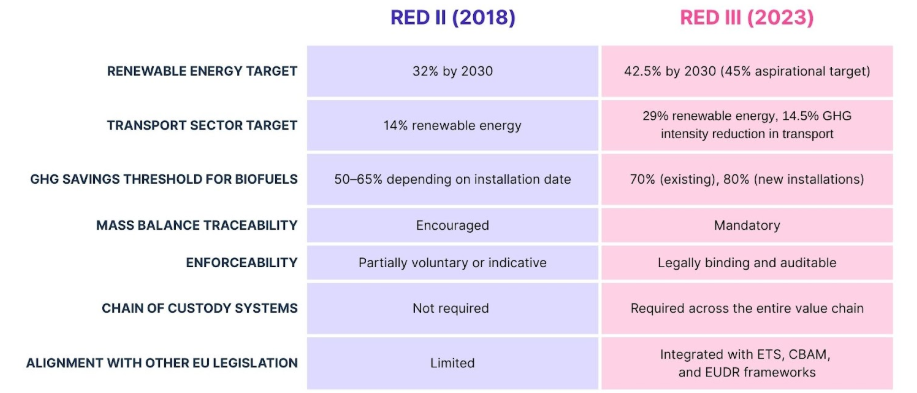
\includegraphics[width=1\linewidth]{red.png}
    \caption{RED 3}
    \label{fig:placeholder}
\end{figure}
\noindent
The initial response to mass EV adoption was characterised by considerable concern within the power sector. The prospect of millions of new electric vehicles was perceived primarily through the lens of risk—vast, temporally correlated loads threatening to overwhelm local distribution networks during peak evening hours. This perspective has undergone a fundamental reassessment. EVs are now recognised not as burdens to be managed, but as essential infrastructure for achieving Europe's energy transition objectives. 
\\
This conceptual shift finds its most concrete expression in \textbf{Vehicle-to-Grid (V2G)} technology, which fundamentally reimagines the role of electric vehicles within the energy system.
\noindent
V2G technology transforms what were previously passive, unidirectional energy consumers into active, distributed, and smart grid resources. The underlying opportunity is both elegant and substantial: private vehicles spend approximately 96\% of their operational lifetime parked and connected \footcite{evertsson2024investigating}, representing an enormous, geographically distributed, and currently underutilised repository of mobile energy storage capacity.
\noindent
The transformative potential of V2G becomes apparent when individual vehicles are coordinated through centrally managed aggregation. While a single EV's contribution remains modest, a carefully orchestrated fleet can function as a unified entity—a \textbf{Virtual Power Plant (VPP)}. These software-defined power plants aggregate the collective capacity of numerous distributed energy resources, delivering grid services at scales and reliability levels comparable to conventional generation facilities. The rapid response characteristics of contemporary battery inverters, operating at millisecond timescales, enable these aggregated fleets to provide a comprehensive range of critical grid services. This capability extends beyond mere utility; it represents a prerequisite for maintaining stability in grids increasingly dependent on the variable and non-dispatchable output of wind and solar generation, thereby enabling the technical and economic viability of the EU's ambitious renewable energy targets \footcite{Tavakoli2019}.
\noindent
The grid services enabled by V2G technology form the technical foundation for the smart, resilient, and decarbonised electricity system required for Europe's energy future:
\\
    \noindent
 \textbf{Frequency Regulation:} Grid stability fundamentally depends on maintaining precise equilibrium between electricity supply and demand, manifested as stable grid frequency (50 Hz across European networks). Frequency deviations signal supply-demand imbalances that, if uncorrected, can trigger cascading failures across interconnected systems. V2G fleets, leveraging their rapid response capabilities, can participate directly in ancillary service markets including Frequency Containment Reserve (FCR) and automatic Frequency Restoration Reserve (aFRR). These systems can inject or absorb power within seconds of frequency deviations, providing immediate counteraction to imbalances and preventing system-wide failures or blackouts \footcite{alfaverh2022optima, white2011vehicle}.
   \\
    \noindent 
\textbf{Demand Response and Peak Shaving:} Through intelligent temporal shifting of charging activities to off-peak periods—when energy is abundant and inexpensive—combined with strategic discharging during peak demand when energy becomes scarce and costly, V2G systems can effectively flatten daily load profiles. This approach directly addresses the "duck curve" phenomenon associated with high solar photovoltaic penetration. Such load profile management reduces dependence on expensive and carbon-intensive "peaker" plants, typically gas or diesel turbine facilities, while potentially deferring or eliminating requirements for costly transmission and distribution infrastructure upgrades \footcite{orfanoudakis2022deep, sadeghi2021deep}.
    \begin{figure}[H]
        \centering
        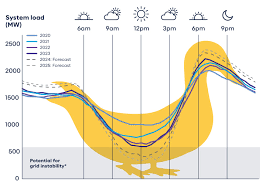
\includegraphics[width=1\linewidth]{duck.png}
        \caption{Duck curve- "La Duck Curve e la scomposizione della stagionalità dei
 consumi elettrici. Aspetti teorici e modelli statistici"-Bisetto Francesca}
        \label{fig:placeholder}
    \end{figure}
    \noindent
  \textbf{Renewable Energy Integration:} The most strategically significant contribution of V2G lies in addressing renewable energy intermittency challenges. V2G fleets function as large-scale energy buffers, absorbing excess solar and wind generation during periods of high production and low demand that would otherwise require curtailment. This stored renewable energy can subsequently be released during periods of low generation, such as evening hours or periods of limited wind availability. This mechanism directly increases the utilisation efficiency of renewable energy resources, supporting the integration objectives outlined in RED III while enhancing overall energy system efficiency \footcite{khan2024review, zou2021deep}.

\noindent
This vision is being actively incorporated into European legal frameworks and technical standards. The transformative \textbf{Alternative Fuels Infrastructure Regulation (AFIR, EU 2023/1804)} now requires that new public charging infrastructure incorporate smart charging capabilities and, critically, bidirectional power flow capacity. The technical implementation of these requirements is supported by standards such as \textbf{ISO 15118-20}, which provides detailed specifications for "Vehicle-to-Grid Communication Interface" (V2GCI) protocols, enabling secure, interoperable bidirectional power transfer. With mandatory implementation scheduled for 2027, the necessary technological and regulatory infrastructure is being systematically established. This regulatory push is supported by significant pilot initiatives including the \textbf{'SCALE'} and \textbf{'V2G Balearic Islands'} projects, which are conducting comprehensive testing of the technology's technical performance and economic viability under real-world operating conditions.

\noindent
Despite this regulatory progress, substantial obstacles to widespread V2G deployment persist. These challenges span technical, economic, and social dimensions:

\begin{itemize}
    \item \textbf{Market and Economic Barriers:} A coherent, pan-European framework for compensating EV owners for grid service provision remains undeveloped. While value streams exist within energy markets, accessing these markets involves significant complexity. Critical issues such as \textbf{"double taxation"} of electricity—where energy faces taxation both during charging and discharging phases—create substantial economic disincentives that require resolution through coordinated policy intervention.
    
    \item \textbf{Regulatory and Grid Access Challenges:} The recognition of EV fleets as qualified flexibility resources varies significantly across national electricity markets. Standardised procedures for grid interconnection, aggregator certification, secure data exchange protocols, and baseline calculation methodologies remain under development, creating a fragmented operational environment that complicates commercial deployment.
    
    \item \textbf{Technical and Consumer Adoption Barriers:} Consumer concerns regarding accelerated \textbf{battery degradation} and its implications for vehicle warranty coverage represent primary obstacles to participation. Additionally, the current installed base of EVs and charging infrastructure lacks universal bidirectional capability, although this limitation is being addressed through new vehicle platforms and evolving charging standards.
\end{itemize}
\noindent
The fundamental challenge addressed by this thesis extends beyond simply enabling V2G technology to encompass its \textit{intelligent orchestration}. This requires developing control strategies sophisticated enough to operate within emerging regulatory frameworks, navigate economic uncertainties, accommodate diverse user preferences, and overcome existing technical constraints. The objective is to unlock the substantial potential of EVs as fundamental components of Europe's energy transition while ensuring system reliability, economic viability, and user acceptance.
%%%%%%%%%%%%%%%%%%%%%%%%%%%%%%
%%%%%%%%%%%%%%%%%%%%%%%%%%%%%%

%%%%%%%%%%%%%%%%%%%%%%%%%%%%%%

%%%%%%%%%%%%%%%%%%%%%%%%%%%%%%


%%%%%%%%%%%%%%%%%%%%%%%%%%%%%%

%%%%%%%%%%%%%%%%%%%%%%%%%%%%%%
\section{The Optimizer's Trilemma: Navigating a Stochastic World}
\begin{center}
  \begin{minipage}{0.85\textwidth}
    \begin{displayquote}
      \large\itshape
      ``Uncertainty quantification provides a systematic way to assess the credibility of computational predictions.''
    \end{displayquote}
  \end{minipage}
\end{center}

\vspace{0.5cm}

\begin{flushright}
  --- \textsc{Omar Ghattas \& Karen Willcox}, \textit{Uncertainty Quantification in Computational Science and Engineering} (2016)
\end{flushright}
\noindent
While the potential of V2G technology is substantial, the management of distributed vehicular assets presents a complex control challenge. Economic viability drives aggregator decisions, yet a narrow focus on profitability alone proves insufficient for sustainable operations. Effective V2G management requires balancing three competing objectives that frequently conflict with one another. This challenge can be framed as the "V2G Optimizer's Trilemma": the concurrent pursuit of \textbf{economic profitability}, preservation of \textbf{battery longevity}, and maintenance of \textbf{user convenience}.
\noindent
Rather than representing a straightforward, static trade-off, this constitutes a dynamic, multi-objective optimisation challenge characterised by \textbf{stochasticity} and \textbf{uncertainty} arising from multiple, interconnected sources \footcite{wang2022multi}:
\\
    \noindent
    \textbf{Market Volatility:} Wholesale electricity prices exhibit significant variability driven by unpredictable supply variations (such as sudden reductions in wind generation capacity) and demand fluctuations (including heat-driven increases in cooling demand). Effective control systems must respond to these price signals dynamically and in real-time.
 \\
    \noindent   
\textbf{Renewable Intermittency:} Co-located solar and wind generation exhibit inherently variable output patterns with limited predictability. Controllers must coordinate EV fleet operations to capture available generation during surplus periods without compromising other operational objectives.
    \\
    \noindent
  \textbf{Human Behaviour:} Perhaps the most challenging uncertainty source involves EV owner patterns. Arrival times, departure schedules, and required state of charge (SoC) at departure lack deterministic characteristics. Emergency departures or unexpected schedule changes represent hard, non-negotiable constraints that intelligent systems must accommodate to preserve user trust and satisfaction.

\noindent
This dynamic, uncertain, and multifaceted operational environment renders static, rule-based control approaches (such as "charge when price falls below threshold X, discharge when exceeding threshold Y") inadequate and brittle. More sophisticated and adaptive methodologies are required—approaches capable of learning from operational experience and making optimal decisions under conditions of significant uncertainty. Reinforcement Learning excels in precisely this domain, providing a framework for developing control policies that demonstrate robustness, adaptability, and scalability.




%%%%%%%%%%%%%%%%%%%%%%%
\subsection{Sources for Energy Price Data}

Access to reliable, real-time, and historical market data remains crucial for both control agent training in simulation environments and real-world deployment. Key public sources for European market data include:
\\
\noindent
 \textbf{ENTSO-E Transparency Platform:} The European Network of Transmission System Operators for Electricity maintains a mandatory, open-access platform serving as a comprehensive repository of pan-European electricity market data. This includes harmonised day-ahead prices, load forecasts, and generation data, serving as the primary source for academic research through both web portal access and free RESTful API services.
    \\
\noindent
    \textbf{National Transmission System Operators (TSOs):} Many national TSOs (including Terna in Italy, National Grid in the UK, and RTE in France) publish detailed market data covering real-time frequency and imbalance prices for their respective jurisdictions.
    \\
\noindent
     \textbf{Power Exchanges:} Exchanges such as \textbf{EPEX SPOT} and \textbf{Nord Pool} constitute actual trading venues. While they represent direct price data sources, comprehensive real-time access typically requires commercial subscription services.


\subsection{Buying vs. Selling: The Critical Retail-Wholesale Spread}
\begin{center}
  \begin{minipage}{0.85\textwidth}
    \begin{displayquote}
      \large\itshape
      ``Price spreads, or marketing margins, are the difference between prices at different stages of the supply chain. 
      The wholesale-to-retail spread is the difference between the wholesale price and the retail price.''
    \end{displayquote}
  \end{minipage}
\end{center}

\vspace{0.5cm}

\begin{flushright}
  --- \textsc{Sebastien Pouliot \& Lee L. Schulz}, \textit{Measuring Price Spreads in Red Meat} (2016)
\end{flushright}
\noindent
A critical yet frequently overlooked aspect of V2G economics involves the distinction between EV owner charging costs and aggregator grid sales revenue.

\begin{itemize}
    \item \textbf{Selling Price (V2G Revenue):} When EVs provide energy to the grid, revenue calculation bases on \textbf{wholesale prices} (such as day-ahead spot prices). These prices reflect pure marginal energy costs at specific times.
    
    \item \textbf{Buying Price (Charging Cost):} End consumer EV charging costs reflect \textbf{retail prices}, significantly exceeding wholesale prices due to numerous non-energy components, termed "non-commodity costs":
    \begin{itemize}
        \item Base wholesale energy costs
        \item \textbf{Grid Tariffs:} Charges for high-voltage transmission and low-voltage distribution network usage
        \item \textbf{Taxes and Levies:} National or regional taxation including VAT and environmental levies applied to electricity consumption
        \item \textbf{Supplier Margin:} Retail energy provider profit margins
    \end{itemize}
\end{itemize}
\noindent
This substantial gap between retail purchasing prices and wholesale selling prices constitutes the "retail-wholesale spread," creating the primary opportunity for profitable energy arbitrage. For instance, with wholesale prices at €50/MWh and retail prices at €250/MWh, arbitrage operations achieve profitability only when selling prices exceed the full €250/MWh acquisition cost, not merely the €50/MWh wholesale component. Successful control strategies must account for these price differentials to enable economically rational decision-making.
\noindent
\\
A further perspective on this issue is provided by Parisio et al. 
\footcite{parisio2014mpc}
(2014), who develop a model predictive control (MPC) framework for microgrid operation. Their formulation explicitly considers the decision of when to buy from or sell to the utility grid, under time-varying spot prices and operational constraints. Importantly, the model prevents physically and economically unrealistic behaviors such as simultaneous buying and selling, and accounts for the real cost of storage and generation. This reinforces the notion that optimal energy management strategies must capture the full set of economic signals—including retail charges, network tariffs, and non-commodity costs—rather than relying solely on wholesale price arbitrage. In the V2G context, this highlights the need for predictive, multi-constraint optimization frameworks capable of managing battery limitations, retail–wholesale spreads, and market participation simultaneously in order to ensure profitability.
\newpage
\section{Modelling the V2G Ecosystem}
\label{sec:ev_and_scenario}

Before examining control algorithms, establishing clear, high-fidelity models of system core components becomes essential: the electric vehicle as a controllable cyber-physical asset, and the operational environment or "scenario." The interaction between these elements defines V2G optimisation task boundaries and objectives.

\subsection{The Grid-Interactive EV as a Controllable Asset}

\begin{center}
  \begin{minipage}{0.85\textwidth}
    \begin{displayquote}
      \large\itshape
      "Electric car sales continue to break records globally, particularly in China and other emerging economies."\\[1em]

    \end{displayquote} 
    
  \end{minipage} 
\end{center}

\begin{flushright}
  \textsc{\textbf{International Energy Agency (IEA)}
\footnote{\href{https://www.iea.org/reports/global-ev-outlook-2025/executive-summary}{Global EV Outlook 2025 - Executive Summary}}}
\end{flushright}



\noindent
From a power grid perspective, electric vehicles represent sophisticated mobile energy storage devices. For V2G applications, EVs can be characterised through several key state variables and parameters:
\\
\noindent
    \textbf{The Battery:} The core grid asset component, defined by \textbf{nominal energy capacity} (in kWh), current \textbf{State of Charge (SoC)}, and \textbf{State of Health (SoH)} representing degradation over time. Operation is constrained by \textbf{power limits} (in kW) dictating maximum charge or discharge rates, and charging/discharging \textbf{efficiencies} accounting for energy losses.
    \\
    \noindent
    \textbf{The On-Board Charger (OBC):} For AC charging applications, the OBC converts grid alternating current to battery direct current. Power rating often constitutes the primary bottleneck for both charging and V2G power output.
    \\
\noindent    
  \textbf{Communication Interface:} V2G participation requires vehicle-charging station (EVSE) communication capabilities. This is governed by standards including \textbf{ISO 15118} and protocols such as the \textbf{Open Charge Point Protocol (OCPP)}, enabling secure information exchange required for smart and bidirectional power flow operations.
\\
\noindent
Combined with vehicle availability patterns—arrival and departure times plus user energy requirements—these characteristics transform EVs from simple loads into fully dispatchable grid resources.
\newpage
%%%%%%%%%%%%%%%%%%%%%%%%%%%%%%%%%%%%%
%%%%%%%%%%%%%%%%%%%%%%%%%%%%%%%%%%%%%%%%
%%%%%%%%%%%%%%%%%%%%%%%%\section{A New Paradigm for Control: Reinforcement Learning}

\section{A New Paradigm for Control: Reinforcement Learning - Based on the work of Sutton \& Barto}



\begin{center}
    \begin{minipage}{0.85\textwidth}
        \large\itshape
        ``Reinforcement learning is learning what to do---how to map situations to actions---so as to maximize a numerical reward signal.''
    \end{minipage}
\end{center}

\vspace{0.5cm}

\begin{flushright}
--- Richard S. Sutton \& Andrew G. Barto, \textit{Reinforcement Learning: An Introduction} (2018) \cite{Sutton2018}
\end{flushright}

\noindent
To address the complexities of uncertainty, multi-objective trade-offs, and dynamic systems, this work employs Reinforcement Learning (RL), a machine learning paradigm that learns optimal sequential decision-making policies through trial-and-error interaction with an environment. Unlike traditional optimal control methods, which depend on an explicit and accurate model of the environment's dynamics, RL agents learn directly from the outcomes of their actions. This model-free approach provides significant robustness in the face of uncertainty and unmodeled dynamics.

\section{The Reinforcement Learning Problem}
The problem of reinforcement learning is formalized as the interaction between a learning \textbf{agent} and its \textbf{environment}. This interaction unfolds over a sequence of discrete time steps, $t = 0, 1, 2, \dots$.

\subsection{The Agent-Environment Interface}
At each time step $t$, the agent receives a representation of the environment's \textbf{state}, $S_t \in \mathcal{S}$, and on that basis selects an \textbf{action}, $A_t \in \mathcal{A}(S_t)$. One time step later, as a consequence of its action, the agent receives a numerical \textbf{reward}, $R_{t+1} \in \mathcal{R}$, and finds itself in a new state, $S_{t+1}$. This interaction loop forms the foundational framework of the RL problem.

\begin{figure}[h!]
    \centering
    % Placeholder for a standard RL interaction diagram
    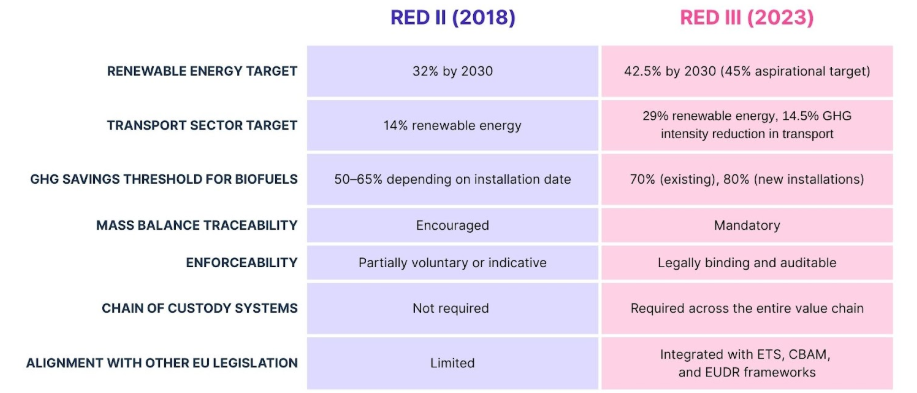
\includegraphics[width=0.8\linewidth]{red.png}
    \caption{The agent-environment interaction loop in reinforcement learning \cite{Sutton2018}.}
    \label{fig:rl_loop}
\end{figure}

\subsection{Goals, Rewards, and Returns}
The agent's objective is formalized by the \textbf{reward hypothesis}: that all goals and purposes can be framed as the maximization of the expected cumulative reward. The agent's goal is not to maximize the immediate reward, $R_{t+1}$, but the cumulative reward in the long run. This cumulative reward is known as the \textbf{return}, denoted $G_t$.

For \textit{episodic tasks} that terminate, the return is the finite sum of future rewards. For \textit{continuing tasks} that do not terminate, the return is defined as the discounted sum of future rewards:
\begin{equation}
    G_t \doteq \sum_{k=0}^{\infty} \gamma^k R_{t+k+1}
\end{equation}
where $\gamma \in [0, 1)$ is the \textbf{discount factor}. It determines the present value of future rewards, ensuring the infinite sum is finite and balancing immediate gratification against long-term gains. A value of $\gamma=0$ results in a myopic agent concerned only with maximizing immediate rewards.

\section{The Language of Learning: Markov Decision Processes}
The mathematical foundation of RL is the \textbf{Markov Decision Process (MDP)}, a formal framework for modeling decision-making in stochastic environments where outcomes are partly random and partly under the control of a decision maker.

\subsection{The Markov Property}
The future is independent of the past given the present. A state signal $S_t$ is said to have the \textbf{Markov Property} if the environment's response at time $t+1$ depends only on the state and action at time $t$. The probability of transitioning to state $s'$ and receiving reward $r$ is independent of all previous states and actions:
\begin{equation}
    p(s', r | s, a) \doteq \Pr\{S_{t+1}=s', R_{t+1}=r | S_t=s, A_t=a\}
\end{equation}
This property is fundamental as it allows decisions to be made based solely on the current state, without needing the complete history of interaction.

\subsection{Policies and Value Functions}
The agent's learning objective is to find a good \textbf{policy}, $\pi(a|s)$, which is a mapping from states to probabilities of selecting each possible action. The goodness of a policy is assessed by its \textbf{value functions}.
\begin{itemize}
    \item The \textbf{state-value function}, $v_\pi(s)$, is the expected return starting from state $s$ and following policy $\pi$ thereafter:
    \begin{equation}
        v_\pi(s) \doteq \mathbb{E}_\pi [G_t | S_t=s]
    \end{equation}
    \item The \textbf{action-value function}, $q_\pi(s, a)$, is the expected return starting from state $s$, taking action $a$, and thereafter following policy $\pi$:
    \begin{equation}
        q_\pi(s, a) \doteq \mathbb{E}_\pi [G_t | S_t=s, A_t=a]
    \end{equation}
\end{itemize}

\section{The Bellman Equations}
The Bellman equations provide a recursive decomposition that is foundational to solving MDPs. They express the value of a state in terms of the values of its successor states.

\subsection{The Bellman Expectation Equation}
For a given policy $\pi$, the state-value function must satisfy a self-consistency condition. The value of a state equals the expected immediate reward plus the discounted expected value of the next state:
\begin{equation}
    v_\pi(s) = \sum_a \pi(a|s) \sum_{s', r} p(s', r | s, a) [r + \gamma v_\pi(s')]
\end{equation}
This is the \textbf{Bellman expectation equation} for $v_\pi$. It forms the basis for policy evaluation algorithms.

\subsection{The Bellman Optimality Equation}
The ultimate goal is to find an \textbf{optimal policy}, $\pi_*$, which is a policy that achieves a higher or equal expected return than all other policies from all states. All optimal policies share the same optimal value functions, $v_*(s)$ and $q_*(s, a)$. The optimal value function for a state is the maximum expected return achievable from that state:
\begin{equation}
    v_*(s) = \max_a \mathbb{E}[R_{t+1} + \gamma v_*(S_{t+1}) | S_t=s, A_t=a] = \max_a \sum_{s', r} p(s', r | s, a) [r + \gamma v_*(s')]
\end{equation}
This is the \textbf{Bellman optimality equation}. Solving it means finding the optimal policy.

\section{Solution Methods: A Unified Perspective}
\subsection{Generalized Policy Iteration (GPI)}
Most RL algorithms can be understood within the framework of \textbf{Generalized Policy Iteration (GPI)}, as described in Chapter 4 of \cite{Sutton2018}. GPI refers to the general idea of letting two interacting processes, policy evaluation and policy improvement, work towards a common optimal solution.

\begin{itemize}
    \item \textbf{Policy Evaluation}: Given a policy $\pi$, compute its value function $v_\pi$. This step aims to make the value function consistent with the current policy.
    \item \textbf{Policy Improvement}: Given a value function $v$, improve the policy by making it greedy with respect to $v$. For a given state $s$, the new policy will select the action $a$ that maximizes $q_\pi(s, a)$.
\end{itemize}

These two processes compete in the short term (improving the policy makes the value function inaccurate) but cooperate in the long term to converge to the optimal policy and optimal value function. \textbf{Dynamic Programming (DP)} methods like policy iteration and value iteration are classic examples of GPI, assuming a perfect model of the environment.

\section{Learning from Experience: MC and TD Methods}
When a model of the environment is not available, we must learn from sampled experience. Chapters 5 and 6 of \cite{Sutton2018} introduce two primary model-free approaches.

\subsection{Monte Carlo (MC) Methods}
MC methods learn value functions by averaging the returns from sample episodes.
\begin{itemize}
    \item \textbf{Principle}: An update to $V(S_t)$ is made only at the end of an episode.
    \item \textbf{Update Target}: The target for the update is the actual, complete return $G_t$.
    \item \textbf{Update Rule} (Constant-$\alpha$): $V(S_t) \leftarrow V(S_t) + \alpha [G_t - V(S_t)]$
    \item \textbf{Properties}: MC methods are unbiased but can have high variance and are only applicable to episodic tasks. They do not \textit{bootstrap}.
\end{itemize}

\subsection{Temporal-Difference (TD) Learning}
TD learning is a central and novel idea in RL, combining ideas from both MC and DP.
\begin{itemize}
    \item \textbf{Principle}: TD methods update the value estimate for a state based on the observed reward and the estimated value of the successor state. They learn from incomplete episodes.
    \item \textbf{Update Target}: The target is an estimate of the return, called the TD Target: $R_{t+1} + \gamma V(S_{t+1})$.
    \item \textbf{Update Rule} (TD(0)): $V(S_t) \leftarrow V(S_t) + \alpha [R_{t+1} + \gamma V(S_{t+1}) - V(S_t)]$
    \item \textbf{Properties}: TD methods \textit{bootstrap}—they update a guess from a guess. This introduces bias but often leads to lower variance and faster learning. They are naturally implemented in an online, fully incremental fashion.
\end{itemize}

\section{Actor-Critic Architectures}
The \textbf{Actor-Critic} architecture provides a powerful and widely adopted method for solving RL problems, particularly in continuous action spaces. It explicitly represents both the policy and the value function using two distinct function approximators (e.g., neural networks).

\begin{itemize}
    \item \textbf{The Critic}: Learns a value function (e.g., $v_\pi(s)$ or $q_\pi(s, a)$). Its role is to evaluate the actor's decisions by computing the TD error:
    \begin{equation}
        \delta_t = R_{t+1} + \gamma V(S_{t+1}) - V(S_t)
    \end{equation}
    \item \textbf{The Actor}: Represents the policy, $\pi_\theta(a|s)$, parameterized by $\theta$. It receives the current state as input and outputs an action. It uses the TD error from the critic as a learning signal to update its parameters via policy gradient methods, improving its strategy over time.
\end{itemize}

This separation of concerns allows for direct policy optimization in continuous or large action spaces while leveraging the stable learning dynamics of TD-based value estimation.
% ===================================================================
% REWARD SHAPING SECTION
% ===================================================================
 \section{Reward Engineering: Shaping Agent Behavior}
\label{sec:reward_shaping}

The reward function is arguably the most critical component in a Reinforcement Learning system. It is the sole mechanism through which a designer can communicate the desired behavior to the agent. A poorly designed reward can lead to unintended and suboptimal behaviors, even if the agent successfully maximizes it. The entire field of reward engineering has become a cornerstone of modern RL, as it is fundamental to applying these algorithms effectively in complex, real-world applications \footcite{ibrahim2024comprehensive}. The V2G problem, with its multiple competing objectives—maximizing profit, ensuring user satisfaction, preserving battery health, and maintaining grid stability—makes reward design particularly challenging. This work explores several sophisticated techniques to guide the learning process effectively.

\subsection{Potential-Based Reward Shaping (PBRS)}
Potential-Based Reward Shaping (PBRS) is perhaps the most theoretically sound method for reward augmentation \footcite{ng1999policy}. It involves adding a shaping term, $F(s, s')$, to the environment's intrinsic reward, $R(s, a, s')$. The new, shaped reward $R'$ is thus defined as:
\[
R'(s, a, s') = R(s, a, s') + F(s, s')
\]
The shaping term itself is defined as the difference between a potential function, $\Phi$, evaluated at the new state and the old state:
\[
F(s, s') = \gamma \Phi(s') - \Phi(s)
\]
where $\gamma$ is the discount factor. The key theoretical guarantee of PBRS is \textbf{policy invariance}: adding a potential-based shaping reward does not change the optimal policy of the underlying MDP. While the agent learns the same optimal behavior, the shaping term can provide dense, intermediate rewards that significantly accelerate the learning process by guiding the agent's exploration.

\subsection{Dynamic and Adaptive Rewards}
Unlike PBRS, which provides a static reward bonus, a dynamic or adaptive reward function can evolve during training. This approach is particularly useful for complex problems where the relative importance of different objectives may change as the agent becomes more competent. For example, an agent could initially be rewarded simply for keeping an EV charged, but as training progresses, the reward function could adapt to introduce penalties for grid overloads or incentives for V2G services \footcite{wan2022dynamic}. This allows the agent to master different facets of the problem sequentially.

\subsection{Curriculum Learning}
While technically a training paradigm rather than a reward modification technique, Curriculum Learning (CL) is highly relevant to reward engineering. CL involves training the agent on a sequence of tasks that gradually increase in difficulty. In the V2G context, an agent might first be trained in a simple scenario with only a few EVs and stable prices. Once it masters this, it is moved to a more complex environment with more EVs, volatile prices, and hard constraints. This structured learning process prevents the agent from being overwhelmed by the full complexity of the problem from the start and can lead to more robust and generalizable policies.

\newpage
\section{The Rise of Deep Reinforcement Learning for V2G Control}

The convergence of RL with the substantial representational capabilities of deep neural networks has given rise to \textbf{Deep Reinforcement Learning (DRL)}, which currently represents the leading edge of V2G control research. The development of DRL algorithms has yielded a comprehensive toolkit, primarily divided into two main families: off-policy and on-policy methods, each exhibiting distinct operational characteristics.
The following figure illustrates the evolutionary relationships between the algorithms that  will be discussed, highlighting how newer ideas were built to overcome the limitations of their predecessors.

\begin{forest}
for tree={
grow=east,
parent anchor=east,
child anchor=west,
edge path={
\noexpand\path [draw] (!u.parent anchor) -- +(-0.5pt,0) |- (.child anchor)\forestoption{edge label};
},
draw,
rounded corners,
align=center,
l sep=7pt,
s sep=4pt,
minimum height=0.4cm,
inner sep=0.1pt,
anchor=west,
}
[RL Methods
[On-Policy
[Policy Gradient
[A2C]
[TRPO\\(Theoretical Stability)
[PPO\\(Practical Simplification)]
]
]
[Gradient-Free
[ARS\\(Random Search)]
]
]
[Off-Policy\\
[DDPG\\(Fundamental)
[DDPG+PER\\(Improve Sampling)]
[TD3\\(Resolve Overestimation)]
[SAC\\(Add Entropy)]
[TQC\\(Distributional Approach)]
]
]
]
\end{forest}
\subsection{Off-Policy Methods: Data-Efficient Learning from Experience}

Off-policy algorithms distinguish themselves through their capacity to learn optimal policies from data generated by different, often more exploratory, behavioral policies. This enables them to reuse historical experiences stored in large \textit{replay buffers}, breaking temporal correlation between experiences and achieving high sample efficiency.

\paragraph{Deep Deterministic Policy Gradient (DDPG)}

A foundational algorithm that successfully extended Deep Q-Networks (DQN) to high-dimensional, continuous action spaces, DDPG represented a significant breakthrough for control problems including V2G \footcite{lillicrap2015continuous}. It employs an actor-critic architecture where the actor deterministically maps states to actions. However, practical applications often encounter substantial training instability and systematic vulnerability to \textbf{overestimation bias}, where critic networks systematically overestimate Q-values, resulting in suboptimal policy learning \footcite{orfanoudakis2022deep, alfaverh2022optima}.

\paragraph{Twin Delayed DDPG (TD3)}

Developed as a direct successor to address DDPG's instabilities, TD3 introduces three key innovations that have become standard in contemporary DRL \footcite{fujimoto2018addressing}. It incorporates (1) clipped double Q-learning, utilizing paired critic networks and selecting minimum estimates to mitigate overestimation bias; (2) delayed policy updates, updating actors less frequently than critics for enhanced stability; and (3) target policy smoothing, adding noise to target actions for learning regularization. These enhancements establish TD3 as a more robust and reliable baseline for complex V2G applications \footcite{liu2023optimal, wang2022multi}.

\paragraph{Soft Actor-Critic (SAC)}

SAC represents a state-of-the-art off-policy algorithm for continuous control, recognized for superior sample efficiency and stability \footcite{haarnoja2019soft}. Its fundamental innovation involves the \textbf{maximum entropy framework}. The agent's objective is modified to maximize both expected reward and policy entropy. This entropy bonus encourages agents to act as randomly as possible while maintaining task success, promoting broader exploration, improved noise robustness, and reduced risk of poor local optima convergence \footcite{logeshwaran2022comparative}.

\paragraph{Truncated Quantile Critics (TQC)}

TQC addresses overestimation bias through a distributional RL approach \footcite{kuznetsov2020controlling}. Rather than learning single expected returns (Q-values), its critic learns complete return probability distributions using quantile regression. By learning multiple return distribution quantiles and truncating the most optimistic quantile estimates before averaging, it provides a more principled and effective method for removing primary overestimation bias sources, frequently achieving superior performance.

\paragraph{Enhancement: Prioritized Experience Replay (PER)}

This represents not a standalone algorithm but a crucial orthogonal modification for off-policy methods. Standard replay buffers sample past transitions uniformly. PER samples transitions based on their "importance," typically proportional to TD error magnitude \footcite{schaul2015prioritized}. This focuses learning processes on surprising or informative experiences, significantly accelerating convergence and improving final performance.

\subsection{On-Policy Methods: Stability through Cautious Updates}

On-policy methods learn exclusively from data generated by current policies being optimized. Once data is used for updates, it is discarded. While this makes them inherently less sample-efficient than off-policy counterparts, their updates often demonstrate greater stability and reduced divergence risk.

\paragraph{Advantage Actor-Critic (A2C/A3C)}

A2C represents a foundational synchronous, on-policy Actor-Critic algorithm. Its powerful extension, \textbf{Asynchronous Advantage Actor-Critic (A3C)}, was a landmark contribution demonstrating parallelism benefits \footcite{mnih2016asynchronous}. A3C utilizes multiple parallel workers, each with individual model and environment copies. These workers interact with their environments independently, and collected gradients update a global model asynchronously. This decorrelates data streams and provides powerful stabilizing effects on learning processes.

\paragraph{Trust Region Policy Optimization (TRPO)}

TRPO was the first algorithm to formalize policy update size constraints for guaranteed monotonic policy improvement \footcite{schulman2020trust}. It maximizes a "surrogate" objective function subject to policy change constraints, measured by Kullback-Leibler (KL) divergence. This creates a "trust region" within which new policies are guaranteed to improve upon previous ones, preventing catastrophic updates that can permanently derail learning. However, implementation complexity arises from second-order optimization requirements.

\paragraph{Proximal Policy Optimization (PPO)}

PPO achieves TRPO's stability benefits and reliable performance using only first-order optimization, making it far simpler to implement and more broadly applicable \footcite{schulman2017proximal}. It employs a novel \textbf{clipping} mechanism in its objective function to discourage large policy updates that would move new policies too far from previous ones, effectively creating "soft" trust regions. Due to its excellent balance of performance, stability, and implementation simplicity, PPO has become a default choice for many on-policy applications.

\subsection{Gradient-Free Methods: An Alternative Path}

\paragraph{Augmented Random Search (ARS)}

As a counterpoint to dominant gradient-based methods, ARS represents a gradient-free approach that optimizes policies directly in parameter space \footcite{mania2018simple}. It operates by exploring random policy parameter perturbations and updating central policy parameter vectors based on observed performance of these perturbations. While often less sample-efficient for complex, high-dimensional problems, its extreme simplicity, scalability, and robustness to noisy rewards can make it competitive in certain domains.

\section{The Model-Based Benchmark: Model Predictive Control (MPC)}

While DRL offers powerful model-free approaches, model based techniques  requires benchmarking against its most robust model-based counterpart: \textbf{Model Predictive Control (MPC)}. MPC originated in the 1970s within the process control industry, with pioneering contributions by Richalet et al. \footcite{Richalet1978ModelPH} and Cutler and Ramaker \footcite{Cutler1980}. The theoretical foundations for stability and optimality were subsequently established rigorously by researchers including Mayne and Rawlings \footcite{mayne2000constraine}.
\noindent
At its core, MPC represents a proactive, forward-looking strategy that employs explicit mathematical system models to predict future evolution. At each control step, it solves finite-horizon optimal control problems to determine optimal control action sequences. Its primary strength, explaining widespread industrial adoption, lies in its inherent capability to proactively handle complex system dynamics and operational constraints \footcite{minchala2025systematic}.
\section{Model Predictive Control Formulation}
\textit{Section based on "Predictive Control for Linear and Hybrid Systems" by F. Borrelli, A. Bemporad, and M. Morari.}

\subsection{The Finite Time Optimal Control Problem}

At each time step $t$, given the current state measurement $x(t)$, a Model Predictive Control (MPC) law is defined by solving a constrained finite time optimal control problem. This is often referred to as Receding Horizon Control (RHC).
\noindent
Consider the discrete-time linear time-invariant system:
\begin{equation}
    x(k+1) = Ax(k) + Bu(k)
\end{equation}
The optimization problem solved at the current time $t$ is formulated as follows, using $x(t)$ as the initial state $x_0$:

\begin{equation}
    J_0^*(x(t)) = \min_{U_0} J_0(x(t), U_0)
\end{equation}
where the cost function $J_0$ for a quadratic objective is defined as:
\begin{equation}
    J_0(x(0), U_0) = x_N' P x_N + \sum_{k=0}^{N-1} (x_k'Qx_k + u_k'Ru_k)
\end{equation}
The minimization is subject to the following constraints for $k=0, \dots, N-1$:
\begin{align}
    \text{subj. to} \quad x_{k+1} &= Ax_k + Bu_k, \\
    x_k &\in \mathcal{X}, \\
    u_k &\in \mathcal{U}, \\
    x_N &\in \mathcal{X}_f, \\
    x_0 &= x(t).
\end{align}
Here, the variables are defined as:
\begin{itemize}
    \item $x_k \in \mathbb{R}^n$ denotes the state vector at time $k$ obtained by starting from the state $x_0 = x(t)$ and applying the input sequence $u_0, \dots, u_{k-1}$.
    \item $U_0 = [u_0', \dots, u_{N-1}']' \in \mathbb{R}^{mN}$ is the decision vector containing all future inputs over the prediction horizon $N$.
    \item $P, Q$ are positive semi-definite state penalty matrices, and $R$ is a positive definite input penalty matrix.
    \item $\mathcal{X} \subseteq \mathbb{R}^n$ and $\mathcal{U} \subseteq \mathbb{R}^m$ are polyhedra representing state and input constraints, respectively.
    \item $\mathcal{X}_f \subseteq \mathbb{R}^n$ is a terminal polyhedral region that the state $x_N$ is constrained to enter.
\end{itemize}

\subsection{The Receding Horizon Policy}

The optimization problem yields an optimal sequence of control inputs $U_0^*(x(t)) = \{u_0^*, u_1^*, \dots, u_{N-1}^*\}$.
In the receding horizon control strategy, only the first element of this sequence is applied to the system:
\begin{equation}
    u(t) = u_0^*(x(t))
\end{equation}
At the next time step, $t+1$, a new state measurement $x(t+1)$ is obtained. The entire optimization problem is then solved again over a shifted horizon $[t+1, t+1+N]$, using $x(t+1)$ as the new initial state. This process is repeated at each sampling instant.


%%%%%%%%%%%%
\subsection{Implicit MPC: Online Optimization}

The most common formulation involves \textbf{Implicit MPC}, where constrained optimization problems are solved online at each control step. For linear systems with quadratic costs, this typically constitutes a Quadratic Program (QP). The controller's objective involves finding future control input sequences 
\[
U = [u_{t|t}, \dots, u_{t+N-1|t}]
\] 
that minimize a cost function $J$ over a prediction horizon $N$.
\noindent
A key insight from \cite{borrelli2017predictive} is that in this formulation, the control law is defined \textbf{implicitly} as the result of an optimization problem. There is no pre-computed algebraic function; the control action is discovered at each step through a numerical computation. This approach is powerful due to its directness but is fundamentally limited by the need to perform this computation online. The authors of \cite{borrelli2017predictive} highlight this on page xii, stating: 
\begin{quote}
“One limitation of MPC is that running the optimization algorithm on-line at each time step requires substantial time and computational resources.”
\end{quote}
\noindent
The finite-horizon optimal control problem is formulated as:
\begin{equation}
\min_{U_t} J(x_t, U_t) = \sum_{k=0}^{N-1} \left( x_{t+k|t}^\top \mathbf{Q} x_{t+k|t} + u_{t+k|t}^\top \mathbf{R} u_{t+k|t} \right) + x_{t+N|t}^\top \mathbf{P} x_{t+N|t}
\end{equation}
where $x_{t+k|t}$ represents the predicted state at future step $k$ based on information at time $t$, and $\mathbf{Q}$, $\mathbf{R}$, and $\mathbf{P}$ are weighting matrices defining trade-offs between state deviation and control effort. This optimization is subject to system dynamics and operational constraints:
\begin{align}
x_{t+k+1|t} &= \mathbf{A} x_{t+k|t} + \mathbf{B} u_{t+k|t} \\
x_{\min} \leq\ &x_{t+k|t} \leq x_{\max} \\
u_{\min} \leq\ &u_{t+k|t} \leq u_{\max}
\end{align}
\noindent
At each time step $t$, this complete problem is solved, but only the first action of the optimal sequence, $u_{t|t}^*$, is applied to the system. The process then repeats at the next time step, $t+1$, using new system state measurements. This feedback mechanism, known as a \textit{receding horizon} strategy, makes MPC robust to disturbances and model mismatch \cite{camacho2013model}.


%%%%%%%%%%%%%%%%%%%%%%
\subsection{Explicit MPC: Offline Pre-computation}

For systems with fast dynamics or limited online computational capacity, \textbf{Explicit MPC} offers an alternative approach. The key idea is to move the computational effort entirely offline. As detailed extensively in \cite{borrelli2017predictive}, this is achieved by treating the current state $x_t$ not as a fixed value, but as a vector of parameters. The constrained optimization problem is then solved offline for all possible initial states within a given range using \textbf{multi-parametric programming}.

\noindent
The authors of \cite{borrelli2017predictive} frame this as the main contribution of their work (Preface, page xii): 
\begin{quote}
“we want to determine the [...] feedback control law $f(x)$ that generates the optimal $u_k = f(x(k))$ \textbf{explicitly} and not just \textbf{implicitly} as the result of an optimization problem.”
\end{quote}
\noindent
The result is not an online algorithm, but a pre-computed, explicit control law, $K(x_t)$, which for linear systems is a \textbf{piecewise affine (PWA) function} of the state vector $x_t$:
\begin{equation}
u^*(x_t) = \mathbf{F}_i x_t + \mathbf{g}_i \quad \text{if } x_t \in \mathcal{X}_i
\end{equation}
\noindent
The state space is partitioned into a set of convex polyhedral regions $\mathcal{X}_i$, with a unique affine control law defined for each region. Online operation is thereby reduced from solving a QP to a simple function evaluation: first, a fast lookup operation identifies which region $\mathcal{X}_i$ the current state $x_t$ occupies, and second, the corresponding simple affine control law is applied. This trades a very high offline computational burden and significant memory requirements for extremely fast and deterministic online execution \cite{bemporad2013explicit, borrelli2017predictive}.

\subsection{Deep Learning for Efficient PWA Representation}

However, this approach suffers from a significant drawback. The number of polyhedral regions, and thus the memory required to store the corresponding affine laws, grows exponentially with the prediction horizon and the number of system constraints \cite{karg2020efficient}. This "curse of dimensionality" severely limits the practical application of traditional Explicit MPC to systems with a small number of states and simple constraints, particularly in memory-constrained embedded applications \cite{karg2020efficient}.
\\
\noindent
To address this limitation, the work in \cite{karg2020efficient} proposes a novel approach for the efficient representation of these PWA control laws using deep learning. The authors demonstrate that a deep neural network utilizing Rectified Linear Unit (ReLU) activation functions is not merely an approximator but can, in fact, \textbf{exactly represent} the PWA function that defines the explicit MPC feedback law. This is based on the key theoretical insight that any PWA function can be decomposed and constructed using simpler elements that have a direct neural network equivalent.
\\
\noindent
The foundation of this exact representation lies in two main results. First, any scalar PWA function $K_i(x_t)$ (representing the $i$-th component of the control vector) can be expressed as the difference of two convex PWA functions \cite{karg2020efficient}:
\begin{equation}
    K_i(x_t) = \gamma_i(x_t) - \eta_i(x_t)
\end{equation}
Second, any convex PWA function, which can be described as the pointwise maximum of a set of affine functions, can be exactly represented by a deep ReLU network. Specifically, a convex function composed of $N$ affine regions can be perfectly modeled by a network with width $n_x + 1$ (where $n_x$ is the dimension of the state space) and depth $N$ \cite{karg2020efficient}.
\\
\noindent
Combining these findings, the complete multi-output MPC control law $K(x_t)$ can be exactly represented by a vector of $n_u$ pairs of deep neural networks, where each pair models the $\gamma_i$ and $\eta_i$ components for a single control output:
\begin{equation}
    K(x_t) = 
    \begin{bmatrix}
        \mathcal{N}(x_t; \theta_{\gamma,1}) - \mathcal{N}(x_t; \theta_{\eta,1}) \\
        \vdots \\
        \mathcal{N}(x_t; \theta_{\gamma,n_u}) - \mathcal{N}(x_t; \theta_{\eta,n_u})
    \end{bmatrix}
\end{equation}
where $\mathcal{N}$ denotes a deep ReLU network with its corresponding set of parameters $\theta$.
\\
\noindent
The particular advantage of using \textit{deep} neural networks lies in their representational efficiency. While the number of parameters (and thus, the memory footprint) of a deep network grows linearly with the number of layers, the number of linear regions it can represent can grow exponentially with its depth \cite{karg2020efficient}. This provides an inverse relationship to the problem of traditional Explicit MPC, allowing a deep network to capture an exponentially large number of control regions with only a modest, linearly growing memory cost.
\\
\noindent
Consequently, this deep learning-based representation transforms the explicit MPC law into a highly compact form. It overcomes the primary obstacle of prohibitive memory requirements, enabling the deployment of complex predictive controllers on embedded systems where storage capacity is a critical constraint \cite{karg2020efficient}.
%%%%%%%
\section{A Comparative Perspective on Control Methodologies}

While DRL represents the cutting edge, contextualizing it within the broader control strategy landscape remains crucial for academic rigor. The choice between learning-based, model-free approaches and optimization-based, model-based approaches represents fundamental philosophical and practical trade-offs.

\begin{table}[H]
\centering
\caption{Comparative Analysis: DRL vs. Model Predictive Control (MPC) for V2G}
\label{tab:drl_vs_mpc}
\resizebox{0.5\textwidth}{!}{
\begin{tabular}{|p{0.2\linewidth}|p{0.35\linewidth}|p{0.35\linewidth}|}
\hline
\textbf{Aspect} & \textbf{Deep Reinforcement Learning (DRL)} & \textbf{Model Predictive Control (MPC)} \\
\hline
\textbf{Paradigm} & Model-Free, learning-based. Learns an optimal policy (a reactive function) via trial-and-error interaction with the environment. & Model-Based, optimisation-based. Solves a constrained optimisation problem at each time step based on a system model and forecasts. \\
\hline
\textbf{Strengths} & \begin{itemize} \item Highly robust to uncertainty and unmodelled stochasticity. \item Does not require an explicit, accurate system model. \item Can learn complex, non-linear control policies. \item Extremely fast inference time (a single forward pass) once trained. \end{itemize} & \begin{itemize} \item Explicitly and rigorously handles hard constraints, providing safety guarantees. \item Proactive and anticipatory if forecasts are accurate. \item Well-established, mature, and theoretically understood. \end{itemize} \\
\hline
\textbf{Weaknesses} & \begin{itemize} \item Can be highly sample-inefficient during the training phase. \item Lacks hard safety guarantees (an active and important area of research). \item The "black box" nature of neural network policies can make them difficult to interpret or verify. \end{itemize} & \begin{itemize} \item Performance is fundamentally shackled to the accuracy of the system model and external forecasts. \item Computationally expensive at each time step, suffering from the "curse of dimensionality" with system size. \item Can be brittle to unexpected forecast errors and unmodelled dynamics. \end{itemize} \\
\hline
\textbf{V2G Suitability} & Excellent for dynamic, highly uncertain environments with complex, non-linear trade-offs and a large number of assets. & Good for problems with simple, well-defined dynamics and reliable forecasts, but struggles with the real-world stochasticity and scale of V2G. \\
\hline
\end{tabular}
}
\end{table}

\noindent
\textbf{Model Predictive Control (MPC)} stands as the most powerful model-based alternative \footcite{alsabbagh2022reinforcement}. Its primary and most compelling strength lies in its native ability to handle hard constraints, which is critical for ensuring safe operation (such as never violating transformer limits or user energy requirements). However, its performance remains fundamentally constrained by the accuracy of its internal model and forecasts of future disturbances (prices, user behavior) \footcite{faggio2023design}. In practice, creating accurate, tractable models for the entire V2G domain proves nearly impossible due to non-linear battery dynamics, extreme market volatility, and the profound unpredictability of human behavior. Furthermore, as EV fleet sizes grow, optimization problem dimensionality explodes, making online computation required at each time step intractable for large fleets \footcite{schwenk2022computationally}.

\noindent
Other methods, such as \textbf{meta-heuristic algorithms} (including genetic algorithms and particle swarm optimization), are sometimes proposed. However, these are typically employed for offline scheduling and lack the real-time, reactive responsiveness required for dynamic V2G control in rapidly changing environments \footcite{kumar2024integration}.

\noindent
Ultimately, DRL's singular advantage lies in its ability to learn and internalize the complex, non-linear trade-offs of multi-objective V2G problems directly from data, without requiring explicit models. This makes it uniquely suited to navigating the profound uncertainties of real-world operations. While other methods have their applications, DRL stands out as the most promising technology for deploying truly intelligent, autonomous, and scalable V2G management systems required to achieve the ambitious energy and climate objectives of the European Union.

\newpage
\section{A Primer on Lithium-Ion Battery Chemistries and Degradation}

The effectiveness, safety, and economic viability of any V2G strategy remain fundamentally constrained by the physical and chemical characteristics of vehicle batteries. Battery chemistry selection dictates EV operational envelopes, influencing energy density, power capabilities, lifespan, and safety profiles. Clear understanding of these trade-offs proves essential for developing robust, realistic, and responsible control algorithms.
\subsection{Fundamental Concepts and Degradation Mechanisms}

Battery degradation is a complex and irreversible process that gradually reduces a cell’s ability to store and deliver energy. It manifests primarily as capacity loss (energy fade) and as an increase in internal resistance (power fade). These phenomena are usually attributed to two categories of mechanisms: \textit{calendar aging} and \textit{cyclic aging} \footcite{birkl2017degradation}.
\noindent   
\\
\textbf{Calendar aging} occurs while the battery is at rest, regardless of whether it is fully charged or nearly empty. The main mechanism behind this process is the slow growth of the \textbf{Solid Electrolyte Interphase (SEI)} layer on the graphite anode. While a thin and stable SEI layer is necessary for battery operation, its continuous thickening consumes both active lithium and electrolyte, resulting in irreversible capacity loss. The rate of SEI growth is particularly sensitive to operating conditions. High temperatures accelerate chemical reaction rates, including parasitic ones, making storage in hot environments detrimental. Similarly, high states of charge (SoC) correspond to low anode potentials, which increase the reactivity of graphite with the electrolyte and foster faster SEI growth \footcite{vetter2005ageing}. For this reason, leaving electric vehicles stored for long periods at 100\% SoC is generally discouraged.
\noindent   
\\
\textbf{Cyclic aging}, in contrast, results from the processes that take place during charging and discharging. This form of degradation is of particular importance for V2G applications, which inherently involve frequent cycling. Several mechanisms contribute to cyclic aging. The repeated intercalation and de-intercalation of lithium ions induce mechanical stress due to the expansion and contraction of electrode materials. Over time, this stress may generate micro-cracks in electrode particles, leading to a loss of electrical contact and a reduction of active material, effects that become more severe with larger \textbf{Depths of Discharge (DoD)}. Mechanical volume changes can also compromise the integrity of the SEI layer, causing cracks that expose fresh anode surface to the electrolyte and trigger renewed SEI growth. In addition, under demanding conditions—such as very high charging rates (high C-rates) or low temperatures—lithium ions may deposit as metallic lithium on the anode surface rather than intercalating properly. This phenomenon, known as lithium plating, is particularly harmful: it leads to rapid capacity loss and may produce dendritic structures capable of piercing the separator, thereby creating internal short circuits and serious safety hazards \footcite{birkl2017degradation}.
\noindent   
\\
Both calendar and cyclic aging are unavoidable, the latter is especially critical for V2G systems. Since these applications require frequent and sometimes deep cycling, understanding and mitigating cyclic degradation is paramount to guarantee long-term system viability.


\subsection{Key Automotive Chemistries}

The EV market is dominated by several key lithium-ion battery families, primarily distinguished by cathode materials. Each chemistry presents different balances of performance characteristics.

\begin{itemize}
    \item \textbf{Lithium Nickel Manganese Cobalt Oxide (NMC):} For years, this has been the most popular choice due to its excellent balance of energy density, power, and cycle life. The ratio of Nickel, Manganese, and Cobalt can be adjusted (such as NMC111, NMC532, NMC811) to prioritize either energy density (high Nickel) or safety and longevity (lower Nickel).
    
    \item \textbf{Lithium Nickel Cobalt Aluminum Oxide (NCA):} Offers very high specific energy (energy density by weight), enabling longer vehicle range. However, it typically comes at the cost of slightly lower cycle life and narrower safety margins compared to NMC, requiring more sophisticated thermal management.
    
    \item \textbf{Lithium Iron Phosphate (LFP):} Is rapidly gaining market share, particularly in standard-range vehicles, due to lower cost (no cobalt, an expensive and ethically contentious material) and superior safety. LFP batteries offer exceptional cycle life (often 3-4 times that of NMC/NCA) and are considered the safest common Li-ion chemistry due to high thermal stability. Their main drawback involves lower energy density.
    
    \item \textbf{Lithium Titanate Oxide (LTO):} This represents a more niche chemistry using titanate-based anodes instead of graphite. This provides exceptional safety (virtually no thermal runaway risk), extremely long cycle life (>10,000 cycles), and excellent low-temperature performance. However, very low energy density and high cost currently limit its use to specialized applications.
\end{itemize}

\subsection{Voltage Profiles and the Challenge of SoC Estimation}

The relationship between battery open-circuit voltage and SoC represents a critical, non-linear function unique to each chemistry. The derivative of cell voltage with respect to DoD, $\frac{dV_{cell}}{d(DoD)}$, constitutes a key parameter for Battery Management Systems (BMS). Steep, monotonic slopes allow BMS to accurately infer SoC from simple voltage measurements. Conversely, flat slopes make this estimation extremely difficult.

\begin{figure}[H]
    \centering
    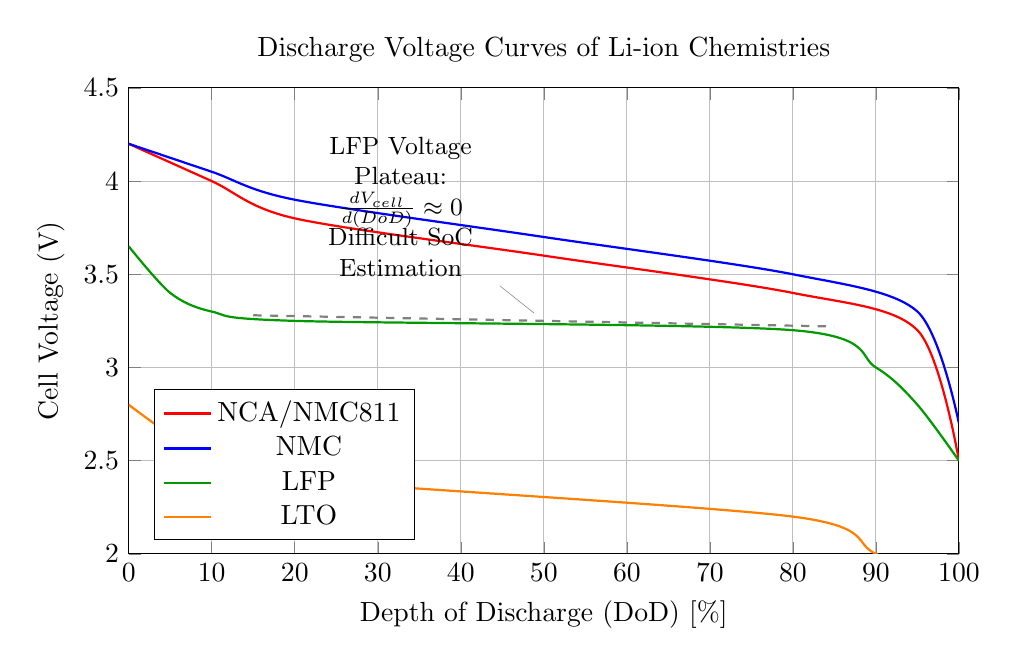
\begin{tikzpicture}
        \begin{axis}[
            title={Discharge Voltage Curves of Li-ion Chemistries},
            xlabel={Depth of Discharge (DoD) [\%]},
            ylabel={Cell Voltage (V)},
            xmin=0, xmax=100,
            ymin=2.0, ymax=4.5,
            grid=major,
            legend pos=south west,
            width=\textwidth,
            height=7.5cm,
        ]
        \addplot[smooth, thick, red] coordinates { (0, 4.2) (10, 4.0) (20, 3.8) (50, 3.6) (80, 3.4) (95, 3.2) (100, 2.5) };
        \addlegendentry{NCA/NMC811}

        \addplot[smooth, thick, blue] coordinates { (0, 4.2) (10, 4.05) (20, 3.9) (50, 3.7) (80, 3.5) (95, 3.3) (100, 2.7) };
        \addlegendentry{NMC}

        \addplot[smooth, thick, green!60!black] coordinates { (0, 3.65) (5, 3.4) (10, 3.3) (20, 3.25) (80, 3.2) (90, 3.0) (95, 2.8) (100, 2.5) };
        \addlegendentry{LFP}
        
        \addplot[smooth, thick, orange] coordinates { (0, 2.8) (10, 2.5) (20, 2.4) (80, 2.2) (90, 2.0) (100, 1.8) };
        \addlegendentry{LTO}

        \draw[dashed, thick, gray] (axis cs:15,3.28) -- (axis cs:85,3.22);
        \node[pin=135:{\parbox{2.5cm}{\centering \small LFP Voltage Plateau: \\ $\frac{dV_{cell}}{d(DoD)} \approx 0$ \\ Difficult SoC Estimation}}] at (axis cs:50,3.25) {};
        \end{axis}
    \end{tikzpicture}
    \caption{Typical discharge voltage curves for various lithium-ion chemistries. The extremely flat profile of LFP makes accurate SoC estimation challenging based on voltage alone, necessitating more complex estimation techniques like Coulomb counting and periodic recalibration\footcite{plett2015battery}.}
    \label{fig:voltage_curves_detailed}
\end{figure}
\noindent
As shown in Figure \ref{fig:voltage_curves_detailed}, LFP's remarkably flat voltage plateau makes it nearly impossible for BMS to determine precise SoC in the central operating range (from approximately 20\% to 80\%) using voltage alone. This necessitates more complex estimation techniques, such as Coulomb counting (integrating current over time), which can suffer from drift. To correct this drift, LFP-equipped vehicles require periodic full charges to 100\% for BMS recalibration. This represents an important operational constraint that V2G control strategies must consider.

\subsection{Comparative Analysis and Safety Considerations}

The trade-offs between chemistries are summarized in Table \ref{tab:chem_comparison_detailed}. Safety remains paramount, with the primary risk being thermal runaway—a dangerous, self-sustaining exothermic reaction. This risk relates directly to cathode material chemical and thermal stability. Higher energy density generally means more energy packed into smaller mass, which can be released violently if cells are compromised. Consequently, critical temperatures for initiating thermal runaway are generally lower for higher energy density chemistries. LFP's stable phosphate-based structure makes it far more resistant to thermal runaway than nickel-based counterparts, a key reason for its growing popularity.

\begin{table}[h!]
\centering
\small
\caption{Comparative analysis of key automotive battery chemistries, highlighting the trade-offs between performance and safety.}
\label{tab:chem_comparison_detailed}
\begin{tabularx}{\textwidth}{
  @{}
  >{\bfseries\RaggedRight}X
  *{5}{C}
  @{}
}
\toprule
Metric & NCA & NMC & LFP & LTO & LCO \\
\midrule
Energy Density (Wh/kg) & 200 - 260 (Highest) & 150 - 220 (High) & 90 - 160 (Moderate) & 60 - 110 (Low) & 150-200 (High) \\
\addlinespace
Cycle Life & 1000 - 2000 & 1000 - 2500 & 2000 - 5000+ & $>$10,000 & 500 - 1000 \\
\addlinespace
Safety & Good & Very Good & Excellent & Excellent & Poor \\
\addlinespace
Thermal Runaway Temp ($^{\circ}$C) & $\sim$150 - 180 & $\sim$180 - 210 & $\sim$220 - 270 & $>$ 250 & $\sim$150 \\
\bottomrule
\end{tabularx}
\end{table}
\clearpage
% ===================================================================
% CHAPTER 3: The EV2Gym Simulation Framework
% ===================================================================
\chapter{An Enhanced V2G Simulation Framework for Robust Control}
\label{chap:ev2gym}

Developing, validating, and benchmarking advanced control algorithms for Vehicle-to-Grid (V2G) systems is a complex endeavor. Real-world experimentation is often impractical due to prohibitive costs, logistical challenges, and risks to grid stability and vehicle hardware. To bridge the gap between theory and practice, a realistic, flexible, and standardized simulation environment is a scientific necessity. This thesis builds upon the foundation of \textbf{EV2Gym}, a state-of-the-art, open-source simulator designed for V2G smart charging research \footcite{orfanoudakis2024ev2gym}. This work, however, extends the original framework significantly, transforming it into a high-fidelity \textbf{digital twin} engineered not just for single-scenario optimization, but for the development and rigorous evaluation of \textbf{robust, generalist control agents}.

This enhanced framework offers a two-pronged approach to experimentation: it allows for deep-dive analysis of agents specialized for a single environment, while also introducing a novel methodology for training and testing agents designed to generalize across a multitude of diverse, unpredictable scenarios. This chapter provides an in-depth tour of this extended architecture, its data-driven models, and its unique evaluation capabilities, establishing the methodological bedrock for the rest of this work.

\section{Core Simulator Architecture}
The framework is built on the modular architecture of EV2Gym, which mirrors the key entities of a real-world V2G system. Its foundation on the OpenAI Gym (now Gymnasium) API is a cornerstone, providing a standardized agent-environment interface defined by the familiar language of states, actions, and rewards \footcite{brockman2016openai}.

The architecture consists of several interacting components:
\begin{itemize}
    \item \textbf{Charge Point Operator (CPO):} The central intelligence of the simulation, managing the charging infrastructure and serving as the primary interface for the control algorithm (the DRL agent). The CPO aggregates system state information and dispatches control actions to individual chargers.
    \item \textbf{Chargers:} Digital representations of physical charging stations, configurable by type (AC/DC), maximum power, and efficiency. This allows for the simulation of heterogeneous charging infrastructures.
    \item \textbf{Power Transformers:} These components model the physical connection points to the grid, aggregating the electrical load from multiple chargers. Crucially, they enforce the physical power limits of the local distribution network and can model inflexible base loads (e.g., buildings) and local renewable generation (e.g., solar panels).
    \item \textbf{Electric Vehicles (EVs):} Dynamic and autonomous agents, each defined by its unique battery capacity, power limits, current and desired energy levels, and specific arrival and departure times.
\end{itemize}
The simulation process follows a reproducible three-phase structure: (1) \textbf{Initialization} from a comprehensive YAML configuration file, (2) a discrete-time \textbf{Simulation Loop} where the agent interacts with the environment, and (3) a final \textbf{Evaluation and Visualization} phase that generates standardized performance metrics.

\section{Core Physical Models}
The simulation's fidelity is anchored in its detailed, empirically validated models, which are essential for developing control strategies robust enough for real-world application.

\subsection{EV Model and Charging/Discharging Dynamics}
The framework implements a realistic two-stage charging/discharging model that captures the non-linear behavior of lithium-ion batteries, simulating both the \textbf{constant current (CC)} and \textbf{constant voltage (CV)} phases. Each EV is defined by a rich parameter set: maximum capacity ($E_{max}$), a minimum safety capacity ($E_{min}$), separate power limits for charging and discharging ($P_{ch}^{max}, P_{dis}^{max}$), and distinct efficiencies for each process ($\eta_{ch}, \eta_{dis}$).

\subsection{Battery Degradation Model}
To address the critical issue of battery health in V2G operations, the simulator incorporates a semi-empirical battery degradation model. It quantifies capacity loss ($Q_{lost}$) as the sum of two primary aging mechanisms \footcite{orfanoudakis2024ev2gym}:
\begin{itemize}
    \item \textbf{Calendar Aging ($d_{cal}$):} Time-dependent capacity loss, influenced by the battery's average State of Charge (SoC) and temperature.
    \item \textbf{Cyclic Aging ($d_{cyc}$):} Wear resulting from charge/discharge cycles, dependent on energy throughput, depth-of-cycle, and C-rate.
\end{itemize}
This integrated model allows for the direct quantification of how different control strategies impact the battery's long-term State of Health (SoH), enabling the training of agents that balance profitability with battery preservation.

\subsection{EV Behavior and Grid Models}
To ensure realism, the simulation is driven by authentic, open-source datasets. EV arrival/departure patterns and energy requirements are modeled using probability distributions derived from a large real-world dataset from \textbf{ElaadNL}. Grid conditions are similarly grounded in reality, using inflexible load data from the \textbf{Pecan Street} project and solar generation profiles from the \textbf{Renewables.ninja} platform \footcite{orfanoudakis2024ev2gym}.

\section{A Unified Experimentation and Evaluation Workflow}
A key contribution of this thesis is the development of a unified and powerful experimentation workflow, orchestrated by the main script \texttt{run\_experiments.py}. This script replaces the previous fragmented approach, providing a single, interactive interface to manage the entire lifecycle of training, benchmarking, and evaluation for V2G control agents. This workflow is designed to be both flexible for research and rigorous for evaluation, supporting the dual goals of developing specialized and generalized agents.

\subsection{Orchestration via \texttt{run\_experiments.py}}
The \texttt{run\_experiments.py} script acts as the central hub for all experimentation. It guides the user through an interactive command-line process, ensuring consistency and reproducibility. The key steps are:
\begin{enumerate}
    \item \textbf{Algorithm Selection:} The user can select from a predefined list of algorithms to benchmark. This includes Deep Reinforcement Learning agents (e.g., SAC, DDPG+PER, TQC), classical optimization methods (Model Predictive Control), and rule-based heuristics (e.g., Charge As Fast As Possible).
    \item \textbf{Scenario Selection:} The script automatically detects all available \texttt{.yaml} configuration files, allowing the user to choose one or more scenarios for the experiment. This choice determines the mode of operation (single-domain vs. multi-scenario).
    \item \textbf{Reward Function Selection:} The framework's flexibility is enhanced by allowing the user to dynamically select the reward function for the RL agents from the \texttt{reward.py} module.
    \item \textbf{Training and Benchmarking:} Based on the user's selections, the script proceeds to the optional training phase and then to a comprehensive benchmark, saving all results in a timestamped directory.
\end{enumerate}

\subsection{Dual-Mode Training: Specialists and Generalists}
The new workflow elegantly unifies the training of both "specialist" and "generalist" agents, a concept previously handled by separate scripts. The behavior is determined implicitly by the number of selected scenarios:
\begin{itemize}
    \item \textbf{Single-Domain Specialization:} If the user selects a single scenario, the script trains an RL agent exclusively on that environment. This produces a specialist agent, optimized to extract maximum performance from a specific, known set of conditions (e.g., a particular charging station topology and price profile).
    \item \textbf{Multi-Scenario Generalization:} If multiple scenarios are selected, the script automatically utilizes the \texttt{MultiScenarioEnv} wrapper. This custom Gymnasium environment dynamically switches between the different selected configurations at the start of each training episode. This process forces the agent to learn a robust and generalizable policy that performs well across a wide range of conditions, preventing overfitting to any single scenario. To handle the technical challenge of varying observation and action space sizes across scenarios, a \texttt{CompatibilityWrapper} is used to pad and slice the state-action vectors, enabling a single neural network policy to control heterogeneous environments.
\end{itemize}

\subsection{Reproducible Benchmarking and Evaluation}
To ensure a fair and scientifically valid comparison, the \texttt{run\_benchmark} function implements a rigorous evaluation protocol. For each scenario, it first generates a "replay" file containing the exact sequence of stochastic events (e.g., EV arrivals, energy demands). This exact same sequence is then used to evaluate every algorithm, eliminating randomness as a factor in performance differences. The script runs multiple simulations for statistical robustness, aggregates the mean results, and automatically generates a suite of comparative plots, including overall performance metrics and detailed battery degradation analyses.

\section{Evaluation Metrics}
To ensure a fair and comprehensive comparison, all algorithms are evaluated against an identical set of pre-generated scenarios through a "replay" mechanism. The \textbf{mean} and \textbf{standard deviation} of performance are calculated across multiple simulation runs. The key metrics include:

\begin{itemize}
    \item \textbf{Total Profit (\$):} The net economic outcome, calculated as revenue from energy sales minus the cost of energy purchases.
    \[
    \Pi_{\text{total}} = \sum_{t=0}^{T_{\text{sim}}} \sum_{i=1}^{N} \left( C_{\text{sell}}(t) P_{\text{dis},i}(t) - C_{\text{buy}}(t) P_{\text{ch},i}(t) \right) \Delta t
    \]
    
    \item \textbf{Tracking Error (RMSE, kW):} For grid-balancing scenarios, this measures the root-mean-square error between the fleet's aggregated power and a target setpoint.
    \[
    E_{\text{track}} = \sqrt{\frac{1}{T_{\text{sim}}} \sum_{t=0}^{T_{\text{sim}}-1} \left( P_{\text{setpoint}}(t) - P_{\text{total}}(t) \right)^2}
    \]
    
    \item \textbf{User Satisfaction (Average):} The fraction of energy delivered compared to what was requested by the user, averaged across all EV sessions. A score of 1 indicates perfect service.
    \[
    US_{\text{avg}} = \frac{1}{N_{\text{EVs}}} \sum_{k=1}^{N_{\text{EVs}}} \min \left(1, \frac{E_k(t_k^{\text{dep}})}{E_k^{\text{des}}} \right)
    \]
    
    \item \textbf{Transformer Overload (kWh):} The total energy that exceeded the transformer's rated power limit. An ideal controller should achieve a value of 0.
    \[
    O_{\text{tr}} = \sum_{t=0}^{T_{\text{sim}}} \sum_{j=1}^{N_T} \max(0, P_j^{\text{tr}}(t) - P_j^{\text{tr,max}}) \cdot \Delta t
    \]
    
    \item \textbf{Battery Degradation (\$):} The estimated monetary cost of battery aging due to both cyclic and calendar effects.
    \[
    D_{\text{batt}} = \sum_{k=1}^{N_{\text{EVs}}} (\text{CyclicCost}_k + \text{CalendarCost}_k)
    \]
\end{itemize}

\section{Simulator Implementation Details}
\label{sec:sim_architecture}
During the analysis and implementation of new metrics, fundamental details about the \texttt{EV2Gym} simulator's architecture emerged, which warrant documentation. The configuration of Electric Vehicles (EVs) and the calculation of their degradation follow a specific logic dependent on a key parameter in the \texttt{.yaml} configuration files.

\subsubsection{Vehicle Definition Modes}
The simulator operates in two distinct modes, controlled by the boolean flag \texttt{heterogeneous\_ev\_specs}:
\begin{itemize}
    \item \textbf{Heterogeneous Mode (\texttt{True}):} In this mode, the simulator ignores the default vehicle specifications in the \texttt{.yaml} file. Instead, it loads a list of vehicle profiles from an external JSON file, specified by the \texttt{ev\_specs\_file} parameter (e.g., \texttt{ev\_specs\_v2g\_enabled2024.json}). This allows for the creation of a realistic fleet with diverse battery capacities, charging powers, and efficiencies. For instance, the fleet may include a \textbf{Peugeot 208} with a 46.3 kWh battery and a 7.4 kW charge rate, alongside a \textbf{Volkswagen ID.4} with a 77 kWh battery and an 11 kW charge rate. A vehicle is randomly selected from this list for each new arrival event.
    \item \textbf{Homogeneous Mode (\texttt{False}):} In this mode, the external JSON file is ignored. All vehicles created in the simulation are identical, and their characteristics are defined exclusively by the \texttt{ev:} block within the \texttt{.yaml} configuration file. The \texttt{battery\_capacity} parameter in this block becomes the single source of truth for the entire fleet.
\end{itemize}

\subsubsection{Empirical Calibration of the Degradation Model}
A significant enhancement in this work is the move towards a more physically representative and flexible battery degradation model. While the underlying semi-empirical model for calendar and cyclic aging remains, the methodology for parameterizing it has been fundamentally improved, addressing previous inconsistencies.

This is achieved through the \texttt{Fit\_battery.py} script, a new utility for empirical model calibration. The script implements the following workflow:
\begin{enumerate}
    \item \textbf{Data Loading:} It loads time-series data from real-world battery aging experiments. The expected data includes measurements of capacity loss over time, along with contextual variables like state of charge (SoC), temperature, and energy throughput.
    \item \textbf{Model Fitting:} Using the \texttt{curve\_fit} function from the SciPy library, the script fits the parameters of the \texttt{Qlost\_model} (which combines calendar and cyclic aging) to the empirical data. This optimization process finds the physical constants (e.g., $\epsilon_0, \zeta_0$) that best explain the observed degradation.
    \item \textbf{Parameter Export:} The script outputs the calibrated parameters. These values can then be used directly in the simulator's configuration, ensuring that the degradation model for a specific EV fleet is grounded in experimental evidence for that battery type.
\end{enumerate}
This calibration workflow, integrated optionally into the main \texttt{run\_experiments.py} script, elevates the simulation's fidelity. It allows the framework to move beyond a single, fixed degradation model (previously calibrated for a 78 kWh battery) and enables the creation of high-fidelity digital twins for a wide variety of EV batteries, provided that the necessary experimental data is available.

\section{Reinforcement Learning Formulation}
The control problem is formalized as a Markov Decision Process (MDP), defined by the tuple $(S, A, P, R, \gamma)$.

\subsection{State Space ($S$)}
The state $s_t \in S$ is a feature vector providing a snapshot of the environment at time $t$. A representative state, as defined in modules like \texttt{V2G\_profit\_max\_loads.py}, includes:
\[
 s_t = [t, P_{\text{total}}(t-1), \mathbf{c}(t, H), \mathbf{L}_1(t, H), \mathbf{PV}_1(t, H), \dots, \mathbf{s}^{\text{EV}}_1(t), \dots, \mathbf{s}^{\text{EV}}_N(t)]^T
\]
where the components are:
\begin{itemize}
    \item $t$: The current time step.
    \item $P_{\text{total}}(t-1)$: The aggregated power from the previous time step.
    \item $\mathbf{c}(t, H)$: A vector of \textbf{predicted future} electricity prices over a horizon $H$.
    \item $\mathbf{L}_j(t, H), \mathbf{PV}_j(t, H)$: Forecasts for inflexible loads and solar generation.
    \item $\mathbf{s}^{\text{EV}}_i(t) = [\text{SoC}_i(t), t^{\text{dep}}_i - t]$: Key information for each EV $i$, including its State of Charge and remaining time until departure.
\end{itemize}

\subsection{Action Space ($A$)}
The action $a_t \in A$ is a continuous vector in $\mathbb{R}^N$, where $N$ is the number of chargers. For each charger $i$, the command $a_i(t) \in [-1, 1]$ is a normalized value that is translated into a power command:
\begin{itemize}
    \item If $a_i(t) > 0$, the EV is charging: $P_i(t) = a_i(t) \cdot P^{\text{max}}_{\text{charge}, i}$.
    \item If $a_i(t) < 0$, the EV is discharging (V2G): $P_i(t) = a_i(t) \cdot P^{\text{max}}_{\text{discharge}, i}$.
\end{itemize}

\subsection{Reward Function}
The reward function $R(t)$ encodes the objectives of the control agent. The framework allows for the selection of different reward functions from the \texttt{reward.py} module to suit various goals. Key examples include:
\begin{itemize}
    \item \textbf{Profit Maximization with Penalties} (\texttt{ProfitMax\_TrPenalty\_UserIncentives}): This function creates a balance between economic gain and physical constraints.
    \[
    R(t) = \underbrace{\text{Profit}(t)}_{\text{Economic Gain}} - \underbrace{\lambda_1 \cdot \text{Overload}(t)}_{\text{Grid Penalty}} - \underbrace{\lambda_2 \cdot \text{Unsatisfaction}(t)}_{\text{User Penalty}}
    \]
    The agent is rewarded for profit but penalized for overloading transformers and for failing to meet the charging needs of departing drivers.
    
    \item \textbf{Squared Tracking Error} (\texttt{SquaredTrackingErrorReward}): Used for grid service applications where precision is paramount.
    \[
    R(t) = - \left( P_{\text{setpoint}}(t) - \sum_{i=1}^N P_i(t) \right)^2
    \]
    The reward is the negative squared error from the power setpoint, incentivizing the agent to minimize this error at all times.
\end{itemize}

By using this enhanced framework, this thesis moves beyond single-scenario optimization to develop and validate an intelligent V2G control agent that is not only high-performing but also robust, adaptable, and ready for the complexities of real-world deployment.

\section{Reinforcement Learning Algorithms}
This work benchmarks several state-of-the-art Deep Reinforcement Learning algorithms. The following sections provide a detailed mathematical description of the selected off-policy, actor-critic algorithms.

\subsubsection{Soft Actor-Critic (SAC)}
SAC is an off-policy actor-critic algorithm designed for continuous action spaces that optimizes a stochastic policy. Its core feature is entropy maximization, which encourages exploration and improves robustness. The agent aims to maximize not only the expected sum of rewards but also the entropy of its policy.

The objective function is:
\[
J(\pi) = \sum_{t=0}^{T} \mathbb{E}_{(s_t, a_t) \sim \rho_\pi} \left[ r(s_t, a_t) + \alpha \mathcal{H}(\pi(\cdot|s_t)) \right]
\]
where $\mathcal{H}$ is the entropy of the policy $\pi$ and $\alpha$ is the temperature parameter, which controls the trade-off between reward and entropy.

SAC uses a soft Q-function, trained to minimize the soft Bellman residual:
\[
L(\theta_Q) = \mathbb{E}_{(s_t, a_t, r_t, s_{t+1}) \sim D} \left[ \left( Q(s_t, a_t) - \left(r_t + \gamma V_{\bar{\psi}}(s_{t+1})\right) \right)^2 \right]
\]
where $D$ is the replay buffer and the soft state value function $V$ is defined as:
\[
V_{\text{soft}}(s_t) = \mathbb{E}_{a_t \sim \pi} [Q_{\text{soft}}(s_t, a_t) - \alpha \log \pi(a_t|s_t)]
\]
To mitigate positive bias, SAC employs two Q-networks (Clipped Double-Q) and takes the minimum of the two target Q-values during the Bellman update.

\subsubsection{Deep Deterministic Policy Gradient + PER (DDPG+PER)}
DDPG is an off-policy algorithm that concurrently learns a deterministic policy $\mu(s | \theta^\mu)$ and a Q-function $Q(s, a | \theta^Q)$. It is the deep-learning extension of the DPG algorithm for continuous action spaces.

\begin{itemize}
    \item \textbf{Critic Update:} The critic is updated by minimizing the mean-squared Bellman error, similar to Q-learning. Target networks ($Q'$ and $\mu'$) are used to stabilize training.
    \[
    L(\theta^Q) = \mathbb{E}_{(s_t, a_t, r_t, s_{t+1}) \sim D} \left[ (y_t - Q(s_t, a_t | \theta^Q))^2 \right]
    \]
    where the target $y_t$ is given by:
    \[
    y_t = r_t + \gamma Q'(s_{t+1}, \mu'(s_{t+1}|
    \theta^{\mu'})|
    \theta^{Q'})
    \]
    \item \textbf{Actor Update:} The actor is updated using the deterministic policy gradient theorem:
    \[
    \nabla_{\theta^\mu} J \approx \mathbb{E}_{s_t \sim D} [\nabla_a Q(s, a | \theta^Q)|_{s=s_t, a=\mu(s_t)} \nabla_{\theta^\mu} \mu(s_t | \theta^\mu)]
    \]
    \item \textbf{Prioritized Experience Replay (PER):} This work enhances DDPG with PER. Instead of uniform sampling from the replay buffer $D$, PER samples transitions based on their TD-error, prioritizing those where the model has the most to learn. The probability of sampling transition $i$ is:
    \[
    P(i) = \frac{p_i^\beta}{\sum_k p_k^\beta}
    \]
    where $p_i = |\delta_i| + \epsilon$ is the priority based on the TD-error $\delta_i$, and $\beta$ controls the degree of prioritization. To correct for the bias introduced by non-uniform sampling, PER uses importance-sampling (IS) weights.
\end{itemize}

\subsubsection{Truncated Quantile Critics (TQC)}
TQC enhances the stability of SAC by modeling the entire distribution of returns instead of just its mean. This is achieved through quantile regression and a novel truncation mechanism to combat Q-value overestimation.

\begin{itemize}
    \item \textbf{Distributional Learning:} TQC employs a set of $N$ critic networks, \{$Q_{\phi_i}(s, a)\}_{i=1}^{N}$, each trained to estimate a specific quantile $\tau_i$ of the return distribution. The target quantiles are implicitly defined as $\tau_i = \frac{i-0.5}{N}$. The critics are trained by minimizing the quantile Huber loss, $L_{QH}$.
    
    \item \textbf{Distributional Target Calculation:} A distributional target is constructed for the Bellman update. First, an action is sampled from the target policy for the next state: $\tilde{a}_{t+1} \sim \pi_{\theta'}(\cdot|s_{t+1})$. Then, a set of $N$ Q-value estimates for the next state is obtained from the $N$ target critic networks: \{$Q_{\phi'_j}(s_{t+1}, \tilde{a}_{t+1})\}_{j=1}^{N}$.
    
    \item \textbf{Truncation:} This is the key idea of TQC. To combat overestimation, the algorithm discards the $k$ largest Q-value estimates from the set of $N$ target values. This truncation removes the most optimistic estimates, which are a primary source of bias, leading to more conservative and stable updates.
    
    \item \textbf{Critic Update:} The target value for updating the $i$-th critic is formed using the Bellman equation with the truncated set of next-state Q-values. The overall critic loss is the sum of the quantile losses across all critics:
    \[
    L(\phi) = \sum_{i=1}^{N} \mathbb{E}_{(s,a,r,s') \sim D} \left[ L_{QH}\left(r + \gamma Q_{\text{trunc}}(s', \tilde{a}') - Q_{\phi_i}(s,a) \right) \right]
    \]
    where $Q_{\text{trunc}}$ represents the value derived from the truncated set of target quantiles.
\end{itemize}



\subsection{A History-Based Adaptive Reward for Profit Maximization}
\label{sec:adaptive_reward}

To effectively steer the learning agent towards a policy that is both highly profitable and reliable, we have designed and implemented a novel, history-based adaptive reward function, named \texttt{FastProfitAdaptiveReward}. This function departs from traditional static-weight penalties and instead introduces a dynamic feedback mechanism where the severity of penalties is directly influenced by the agent's recent performance. The core philosophy is to aggressively prioritize economic profit while using adaptive penalties as guardrails that become stricter only when the agent begins to consistently violate operational constraints.

The total reward at each timestep $t$, $R_t$, is calculated as the net economic profit minus any active penalties for user dissatisfaction or transformer overload.

\begin{equation}
    R_t = \Pi_t - P_t^{\text{sat}} - P_t^{\text{tr}}
\end{equation}

\subsubsection{Economic Profit}
The foundation of the reward signal is the direct, instantaneous economic profit, $\Pi_t$. This component provides a clear and strong incentive for the agent to learn market dynamics, encouraging it to charge during low-price periods and discharge (V2G) during high-price periods.
\begin{equation}
    \Pi_t = \sum_{i=1}^{N} \left( C_t^{\text{sell}} \cdot P_{i,t}^{\text{dis}} - C_t^{\text{buy}} \cdot P_{i,t}^{\text{ch}} \right) \Delta t
\end{equation}
where $N$ is the number of connected EVs, $C_t^{\text{sell}}$ and $C_t^{\text{buy}}$ are the electricity prices, and $P_{i,t}^{\text{dis}}$ and $P_{i,t}^{\text{ch}}$ are the discharging and charging powers for EV $i$.

\subsubsection{Adaptive User Satisfaction Penalty}
The penalty for failing to meet user charging demands, $P_t^{\text{sat}}$, is not a fixed value. Instead, it adapts based on the system's recent history of performance. The environment maintains a short-term memory of the average user satisfaction over the last 100 timesteps. From this history, we calculate an average satisfaction score, $\bar{S}_{hist}$.

A \textit{satisfaction severity multiplier}, $\lambda_t^{\text{sat}}$, is then calculated. This multiplier grows quadratically as the historical average satisfaction drops, meaning that if the system has been performing poorly, the consequences for a new failure become much more severe.
\begin{equation}
    \lambda_t^{\text{sat}} = \lambda_{\text{base}}^{\text{sat}} \cdot (1 - \bar{S}_{hist})^2
\end{equation}
where $\lambda_{\text{base}}^{\text{sat}}$ is a base scaling factor (e.g., 20.0). A penalty is only applied if any departing EV's satisfaction, $S_k$, is below a critical threshold (e.g., 95\%). The magnitude of the penalty is the product of the adaptive multiplier and the current satisfaction deficit.
\begin{equation}
    P_t^{\text{sat}} = \lambda_t^{\text{sat}} \cdot (1 - \min(S_k)) \quad \forall k \in \text{EVs departing at } t
\end{equation}
This creates a powerful feedback loop: a single, isolated failure in an otherwise well-performing system results in a mild penalty. However, persistent failures lead to a rapidly escalating penalty, forcing the agent to correct its behavior.

\subsubsection{Adaptive Transformer Overload Penalty}
Similarly, the transformer overload penalty, $P_t^{\text{tr}}$, adapts based on the recent frequency of overloads. The environment tracks how often an overload has occurred in the last 100 timesteps, yielding an overload frequency, $F_{hist}^{\text{tr}}$.

This frequency is used to compute a linear \textit{overload severity multiplier}, $\lambda_t^{\text{tr}}$. The more frequently overloads have happened, the higher the penalty for a new one.
\begin{equation}
    \lambda_t^{\text{tr}} = \lambda_{\text{base}}^{\text{tr}} \cdot F_{hist}^{\text{tr}}
\end{equation}
where $\lambda_{\text{base}}^{\text{tr}}$ is a base scaler (e.g., 50.0). If the total power drawn, $P_j^{\text{total}}(t)$, exceeds the transformer's limit, $P_j^{\text{max}}$, a penalty is applied. This penalty consists of a small, fixed base amount plus the adaptive component, which scales with the magnitude of the current overload.
\begin{equation}
    P_t^{\text{tr}} = P_{\text{base}} + \lambda_t^{\text{tr}} \cdot \sum_{j=1}^{N_T} \max(0, P_j^{\text{total}}(t) - P_j^{\text{max}})
\end{equation}
This mechanism teaches the agent that while a rare, minor overload might be acceptable in pursuit of high profit, habitual overloading is an unsustainable and heavily penalized strategy.

\subsubsection{Rationale and Significance}
This history-based adaptive reward function represents a significant advancement over static or purely state-based approaches. By making the penalty weights a function of the system's recent performance history, we provide a more nuanced and stable learning signal. The agent is not punished excessively for isolated, exploratory actions that might lead to a minor constraint violation. Instead, it is strongly discouraged from developing policies that lead to chronic system failures.

The intuition is to mimic a more realistic management objective: maintain high performance on average, and react strongly only when performance trends begin to degrade. This method is also computationally efficient, avoiding complex state-dependent calculations in favor of simple updates to historical data queues. Ultimately, this reward structure guides the agent to discover policies that are not only profitable but also robust and reliable over time, striking a more intelligent balance between economic ambition and operational safety.


\newpage
\section{Model Predictive Control (MPC)}
The MPC, implemented in \texttt{mpc.py} and \texttt{eMPC.py}, solves an optimization problem at every time step over a prediction horizon $H$.

\subsection{System Model}
The system is modeled in linear state-space form. The state $\mathbf{x}_k \in \mathbb{R}^N$ is the vector of SoCs of all EVs at time $k$. The input $\mathbf{u}_k \in \mathbb{R}^{2N}$ is the vector of charging and discharging powers.
\[
\mathbf{x}_{k+1} = A_k \mathbf{x}_k + B_k \mathbf{u}_k
\]
The matrices $A_k$ (\texttt{Amono}) and $B_k$ (\texttt{Bmono}) are time-varying because they depend on which EVs are connected. $A_k$ is typically a diagonal identity-like matrix modeling the persistence of EVs. $B_k$ maps power to SoC change, including efficiencies and $\Delta t$.

\subsection{Optimization Problem}
At time $t$, the MPC solves:
\[
\min_{\{\mathbf{u}_k\}_{k=t}^{t+H-1}} \sum_{k=t}^{t+H-1} \mathbf{f}_k^T \mathbf{u}_k
\]
subject to:
\begin{align*}
    & \mathbf{x}_{k+1} = A_k \mathbf{x}_k + B_k \mathbf{u}_k, \quad \forall k \in [t, t+H-1] & \text{(Dynamics)} \\
    & \mathbf{x}^{\text{min}}_k \le \mathbf{x}_k \le \mathbf{x}^{\text{max}}_k & \text{(SoC limits)} \\
    & \mathbf{0} \le \mathbf{u}^{\text{ch}}_k \le \mathbf{u}^{\text{ch,max}}_k \cdot \mathbf{z}_k & \text{(Charge limits)} \\
    & \mathbf{0} \le \mathbf{u}^{\text{dis}}_k \le \mathbf{u}^{\text{dis,max}}_k \cdot (1 - \mathbf{z}_k) & \text{(Discharge limits)} \\
    & \sum_{i \in \text{CS}_j} (u^{\text{ch}}_i - u^{\text{dis}}_i) + L_j(k) - PV_j(k) \le P_j^{\text{tr,max}}(k) & \text{(Transformer limits)}
\end{align*}
where $\mathbf{z}_k$ is a vector of binary variables to prevent simultaneous charge and discharge. The cost vector $\mathbf{f}_k$ contains the energy prices. The code formulates this problem compactly as $\mathbf{AU} \le \mathbf{bU}$, where $\mathbf{U}$ is the vector of all actions over the horizon.

\section{Offline Optimization with Gurobi}
Gurobi is used to find the optimal offline (a posteriori) solution, providing a performance benchmark. The files \texttt{profit\_max.py} and \texttt{tracking\_error.py} define the optimization problem over the entire simulation horizon $T_{\text{sim}}$.

\subsection{Decision Variables}
\begin{itemize}
    \item $E_{p,i,t}$: Energy in the EV at port $p$ of station $i$ at time $t$.
    \item $I^{\text{ch}}_{p,i,t}, I^{\text{dis}}_{p,i,t}$: Charging/discharging currents.
    \item $\omega^{\text{ch}}_{p,i,t}, \omega^{\text{dis}}_{p,i,t}$: Binary variables for operating modes.
\end{itemize}

\subsection{Objective Function (Example: Profit Maximization)}
\[
\max \sum_{t=0}^{T_{\text{sim}}} \sum_{i=1}^{N_{CS}} \sum_{p=1}^{N_p} \left( C_{\text{sell}}(t) P^{\text{dis}}_{p,i,t} - C_{\text{buy}}(t) P^{\text{ch}}_{p,i,t} \right) \Delta t - \lambda \sum_{k \in \text{EVs departed}} (E_k^{\text{des}} - E_k(t_k^{\text{dep}}))^2
\]
where $P = V \cdot I \cdot \eta$.

\subsection{Main Constraints}
\begin{itemize}
    \item \textbf{Energy Balance:}
    \[
    E_{p,i,t} = E_{p,i,t-1} + (\eta_{\text{ch}} V_i I^{\text{ch}}_{p,i,t} - \frac{1}{\eta_{\text{dis}}} V_i I^{\text{dis}}_{p,i,t}) \Delta t
    \]
    \item \textbf{Activation of Current:}
    \[
    I^{\text{ch}}_{p,i,t} \le M \cdot \omega^{\text{ch}}_{p,i,t} \quad , \quad I^{\text{dis}}_{p,i,t} \le M \cdot \omega^{\text{dis}}_{p,i,t}
    \]
    \item \textbf{Mutual Exclusion:}
    \[
    \omega^{\text{ch}}_{p,i,t} + \omega^{\text{dis}}_{p,i,t} \le 1
    \]
    \item \textbf{Current and SoC Limits:}
    \[
    I^{\text{min}} \le I_{p,i,t} \le I^{\text{max}} \quad , \quad E^{\text{min}} \le E_{p,i,t} \le E^{\text{max}}
    \]
    \item \textbf{SoC at Departure:}
    \[
    E_{p,i}(t^{\text{dep}}) \ge E^{\text{des}}_{p,i}
    \]
\end{itemize}
\section{Online MPC Formulation (PuLP Implementation)}

The Model Predictive Control (MPC) implemented with PuLP solves a profit maximization problem at each time step $t$ over a finite prediction horizon $H$. This formulation is designed for online, real-time control, where decisions are made based on the current system state and future predictions.

\subsection{Mathematical Formulation}
At each time step $t$, the MPC controller solves the following optimization problem.

\subsubsection{Objective Function: Net Operational Profit}
The objective is to maximize the total net operational profit over the control horizon $H$. This provides a comprehensive economic model that goes beyond simple energy arbitrage.
\begin{equation}
\max_{P^{\text{ch}}, P^{\text{dis}}, z} \sum_{k=t}^{t+H-1} \sum_{i \in \text{CS}} \left( \text{Revenues}_{i,k} - \text{Costs}_{i,k} \right)
\end{equation}
The revenue and cost components are defined for each station $i$ at time step $k$ as:
\begin{itemize}
    \item \textbf{Revenues} consist of:
    \begin{itemize}
        \item Grid Sales Revenue (V2G): $c^{\text{sell}}_k \cdot P^{\text{dis}}_{i,k} \cdot \Delta t$
        \item User Charging Revenue: $c^{\text{user}} \cdot P^{\text{ch}}_{i,k} \cdot \Delta t$
    \end{itemize}
    \item \textbf{Costs} consist of:
    \begin{itemize}
        \item Grid Purchase Cost: $c^{\text{buy}}_k \cdot P^{\text{ch}}_{i,k} \cdot \Delta t$
        \item Battery Degradation Cost: $c^{\text{deg}} \cdot (P^{\text{ch}}_{i,k} + P^{\text{dis}}_{i,k}) \cdot \Delta t$
    \end{itemize}
\end{itemize}
where $c^{\text{sell}}_k$ and $c^{\text{buy}}_k$ are the time-varying electricity prices, $c^{\text{user}}$ is the fixed price for the end-user, $c^{\text{deg}}$ is the estimated cost of battery degradation per kWh cycled, and $\Delta t$ is the time step duration.

\subsubsection{System Constraints}
The optimization is subject to the following constraints for each station $i$ and time step $k \in [t, t+H-1]$.

\paragraph{Energy Balance Dynamics.} The state of energy of the EV battery evolves according to:
\begin{equation}
E_{i,k} = E_{i,k-1} + \left( \eta^{\text{ch}} P^{\text{ch}}_{i,k} - \frac{1}{\eta^{\text{dis}}} P^{\text{dis}}_{i,k} \right) \cdot \Delta t
\end{equation}
where the initial state $E_{i,t-1}$ is the currently measured energy level of the EV.

\paragraph{Power Limits and Mutual Exclusion.} Charging and discharging powers are bounded by the EV's capabilities and controlled by a binary variable $z_{i,k}$ to prevent simultaneous operation.
\begin{align}
    0 &\le P^{\text{ch}}_{i,k} \le P^{\text{ch,max}}_{i} \cdot z_{i,k} \\
    0 &\le P^{\text{dis}}_{i,k} \le P^{\text{dis,max}}_{i} \cdot (1 - z_{i,k})
\end{align}

\paragraph{State of Energy (SoE) Limits.} The battery energy level must remain within its physical operational window.
\begin{equation}
E^{\text{min}}_{i} \le E_{i,k} \le E^{\text{max}}_{i}
\end{equation}

\paragraph{User Satisfaction (Hard Constraint).} The desired energy level must be met at the time of departure. This is modeled as a hard constraint, reflecting a non-negotiable service requirement.
\begin{equation}
E_{i,k_{\text{dep}}} \ge E^{\text{des}}_{i}
\end{equation}
where $k_{\text{dep}}$ is the predicted departure step of the EV within the horizon.

\paragraph{Transformer Power Limit.} The total net power drawn from (or injected into) the grid by all charging stations must not exceed the transformer's maximum capacity.
\begin{equation}
\sum_{i \in \text{CS}} (P^{\text{ch}}_{i,k} - P^{\text{dis}}_{i,k}) \le P^{\text{tr,max}}
\end{equation}


\section{Approximate Explicit MPC: A Machine Learning Approach}
The online, implicit MPC formulation provides high-quality control decisions by solving an optimization problem at every time step. However, this approach has a significant drawback: its computational complexity. For scenarios with a large number of EVs or a long control horizon, solving a Mixed-Integer Linear Program (MILP) in real-time can be prohibitively slow, making it impractical for many real-world applications.

To overcome this limitation, this work implements an \textbf{Approximate Explicit Model Predictive Controller (A-MPC)}. This controller leverages machine learning to replace the computationally expensive online optimization with a fast, lightweight inference step.

\subsection{Methodology: From Oracle to Apprentice}
The core idea is to treat the slow but powerful online MPC as an "oracle" or expert teacher. An apprentice model, in this case a \texttt{RandomForestRegressor} from the \texttt{scikit-learn} library, is trained to mimic the oracle's behavior. The process is as follows:
\begin{enumerate}
    \item \textbf{Data Generation:} The online MPC is run across a diverse range of simulated scenarios. At each step, the state of the environment and the corresponding optimal action computed by the MPC are recorded. This creates a large dataset of state-action pairs, where the actions are considered to be the "ground truth" optimal decisions.
    \item \textbf{State Vector Formulation:} The state $s_t$ fed to the machine learning model is a carefully crafted vector that summarizes all necessary information for making a control decision. It is a fixed-size vector composed of:
    \begin{equation}
        s_t = [ \mathbf{SoC}, \mathbf{T}^{\text{rem}}, \mathbf{C}^{\text{ch}}, \mathbf{C}^{\text{dis}} ]^T
    \end{equation}
    where:
    \begin{itemize}
        \item $\mathbf{SoC}$: A vector of the current State of Charge for all charging stations (padded to a maximum size).
        \item $\mathbf{T}^{\text{rem}}$: A vector of the remaining time until departure for each connected EV.
        \item $\mathbf{C}^{\text{ch}}$: A vector of predicted future charging prices over the horizon $H$.
        \item $\mathbf{C}^{\text{dis}}$: A vector of predicted future discharging prices over the horizon $H$.
    \end{itemize}
    \item \textbf{Offline Training:} The \texttt{RandomForestRegressor} model, denoted $f_{\theta}$, is trained offline on this dataset to learn the mapping from a given state $s_t$ to the oracle's action $a_t$. The model's parameters $\theta$ are optimized to minimize the difference between its predicted action and the oracle's action.
    \item \textbf{Online Inference:} Once trained, the A-MPC controller can be deployed. At each time step, it simply constructs the state vector $s_t$ and computes the action via a fast forward pass through the trained model:
    \begin{equation}
        a_t = f_{\theta}(s_t)
    \end{equation}
    This inference step is orders of magnitude faster than solving a MILP, enabling real-time control for large-scale systems.
\end{enumerate}

\section{Lyapunov-based Adaptive Horizon MPC}
While the A-MPC offers a significant speed-up, it is an approximation and may not always match the performance of the fully-fledged online MPC. A second enhancement developed in this work is the \textbf{Lyapunov-based Adaptive Horizon MPC}, which aims to reduce the computational burden of the online MPC while retaining its optimality and stability guarantees. This method represents an essential improvement, creating an intelligent trade-off between computational cost and control performance.

\subsection{Core Concept: Dynamic Horizon Adjustment}
The key insight is that a long prediction horizon is not always necessary. When the system is in a stable state and far from its operational constraints, a shorter horizon is sufficient for making good decisions. Conversely, when the system is in a complex or critical state (e.g., an EV is close to its departure time but has a low SoC), a longer horizon is needed for careful planning.

This adaptive controller dynamically adjusts its prediction horizon $H_t$ at each step based on the stability of the system, which is formally assessed using a Lyapunov function.

\subsection{Lyapunov Stability for V2G Control}
A Lyapunov function $V(x)$ is a scalar function that can be thought of as a measure of the system's "energy" or deviation from a desired equilibrium state. For the V2G system, we define the state as the vector of energy levels of all connected EVs, $E = [E_1, E_2, \dots, E_N]^T$. The desired state is the vector of desired energy levels at departure, $E^{\text{des}}$. The Lyapunov function is defined as the sum of the squared errors from this desired state:
\begin{equation}
    V(E) = \sum_{i \in \text{EVs}} (E_i - E_i^{\text{des}})^2
\end{equation}
For the system to be stable, the value of this function must decrease at each step, ensuring the system is always progressing towards its goal. This is known as the Lyapunov decrease condition:
\begin{equation}
    V(E_{t+1}) \le V(E_t) - \alpha V(E_t)
\end{equation}
where $E_{t+1}$ is the state at the next time step resulting from the current control action, and $\alpha$ is a small positive constant that sets the minimum required rate of convergence.

\subsection{Horizon Shortening and Extension}
The adaptive MPC algorithm uses this stability condition to govern its horizon length. At each time step $t$:
\begin{enumerate}
    \item The MPC solves the optimization problem using its current horizon, $H_t$.
    \item It calculates the predicted next state $E_{t+1}$ based on the computed optimal action.
    \item It checks if the Lyapunov decrease condition is satisfied.
    \begin{itemize}
        \item \textbf{If Stable:} The condition holds. The controller is performing well. We can afford to reduce the computational load for the next step by shortening the horizon:
        \begin{equation}
            H_{t+1} = \max(H_{\min}, H_t - 1)
        \end{equation}
        \item \textbf{If Not Stable:} The condition is violated. The system requires more careful planning. The horizon for the next step is extended to provide a longer view into the future:
        \begin{equation}
            H_{t+1} = \min(H_{\max}, H_t + 1)
        \end{equation}
    \end{itemize}
\end{enumerate}
This intelligent adjustment makes the online MPC more efficient and practical, reducing computation time during stable periods while retaining the ability to perform deep planning when necessary.

\clearpage

% ===================================================================
% BIBLIOGRAPHY
% ===================================================================


\printbibliography
\end{document}